% Chapter 15: Review and exam preparation
% Time Series Analysis -- Bachelor's programmes Economic Informatics and Economic Cybernetics, Bucharest University of Economic Studies
% GENERATED by latex/build_chapter15.py -- edit the generator, not this file.

\newcommand{\coursename}{Time Series Analysis}
% Preambul comun TSA -- Serii de timp / Time Series Analysis (Beamer, 16:9)
% Același design ca MFM și SFM (preluat din SFM, 5 octombrie 2026). Înainte de % Preambul comun TSA -- Serii de timp / Time Series Analysis (Beamer, 16:9)
% Același design ca MFM și SFM (preluat din SFM, 5 octombrie 2026). Înainte de % Preambul comun TSA -- Serii de timp / Time Series Analysis (Beamer, 16:9)
% Același design ca MFM și SFM (preluat din SFM, 5 octombrie 2026). Înainte de \input{../../latex/preamble} se definește
%   \newcommand{\coursename}{Time Series Analysis}      (EN)
%   \newcommand{\coursename}{Serii de timp}       (RO)  și  \def\tsalang{ro}
% Fișierele .tex se află în EN/Courses, EN/Seminars, RO/Cursuri, RO/Seminarii (două niveluri sub rădăcină).
% Deck-urile sînt generate de latex/build_chapterN.py / build_seminarN.py (vezi latex/tsa_build.py).

\documentclass[9pt, aspectratio=169, t]{beamer}
\providecommand{\coursename}{Time Series Analysis}

% Ensure content fits on slides
\setbeamersize{text margin left=8mm, text margin right=8mm}
% Smaller institute font (title page)
\setbeamerfont{institute}{size=\footnotesize}

%=============================================================================
% THEME AND STYLE CONFIGURATION
%=============================================================================
\usetheme{default}
% Using default theme for clean header/footer control

% Color Palette (matching Redispatch PDF)
\definecolor{MainBlue}{RGB}{26, 58, 110}
\definecolor{AccentBlue}{RGB}{26, 58, 110}
\definecolor{IDAred}{RGB}{205, 0, 0}
\definecolor{DarkGray}{RGB}{51, 51, 51}
\definecolor{MediumGray}{RGB}{128, 128, 128}
\definecolor{LightGray}{RGB}{248, 248, 248}
\definecolor{VeryLightGray}{RGB}{235, 235, 235}
\definecolor{KeynoteGray}{RGB}{218, 218, 218}
\definecolor{SectionGray}{RGB}{120, 120, 120}
\definecolor{FooterGray}{RGB}{100, 100, 100}
\definecolor{Crimson}{RGB}{220, 53, 69}
\definecolor{Forest}{RGB}{46, 125, 50}
\definecolor{Amber}{RGB}{181, 133, 63}
\definecolor{Orange}{RGB}{230, 126, 34}
\definecolor{Purple}{RGB}{142, 68, 173}

% Gradient background (exact Keynote 315° gradient: white to RGB 218,218,218)
\setbeamertemplate{background}{%
    \begin{tikzpicture}[remember picture, overlay]
        \shade[shading=axis, shading angle=315,
        top color=white, bottom color=KeynoteGray]
        (current page.south west) rectangle (current page.north east);
    \end{tikzpicture}%
}
% Fallback solid color for compatibility
\setbeamercolor{background canvas}{bg=}

\setbeamercolor{palette primary}{bg=MainBlue, fg=white}
\setbeamercolor{palette secondary}{bg=MainBlue!85, fg=white}
\setbeamercolor{palette tertiary}{bg=MainBlue!70, fg=white}
\setbeamercolor{structure}{fg=MainBlue}
\setbeamercolor{title}{fg=IDAred}
\setbeamercolor{frametitle}{fg=IDAred, bg=}
\setbeamercolor{block title}{bg=MainBlue, fg=white}
\setbeamercolor{block body}{bg=VeryLightGray, fg=DarkGray}
\setbeamercolor{block title alerted}{bg=Crimson, fg=white}
\setbeamercolor{block body alerted}{bg=Crimson!8, fg=DarkGray}
\setbeamercolor{block title example}{bg=Forest, fg=white}
\setbeamercolor{block body example}{bg=Forest!8, fg=DarkGray}
\setbeamercolor{item}{fg=MainBlue}

% Footer colors (override Madrid theme blue)
\setbeamercolor{author in head/foot}{fg=FooterGray, bg=}
\setbeamercolor{title in head/foot}{fg=FooterGray, bg=}
\setbeamercolor{date in head/foot}{fg=FooterGray, bg=}
\setbeamercolor{section in head/foot}{fg=FooterGray, bg=}
\setbeamercolor{subsection in head/foot}{fg=FooterGray, bg=}

% Bullet styles (apply everywhere including blocks)
\setbeamertemplate{itemize item}{\color{MainBlue}$\boxdot$}
\setbeamertemplate{itemize subitem}{\color{MainBlue}$\blacktriangleright$}
\setbeamertemplate{itemize subsubitem}{\color{MainBlue}\tiny$\bullet$}
\setbeamertemplate{itemize/enumerate body begin}{\normalsize}
\setbeamertemplate{itemize/enumerate subbody begin}{\normalsize}

% Item spacing - compact style
\setlength{\leftmargini}{10pt}       % Level 1: minimal indent
\setlength{\leftmarginii}{10pt}      % Level 2: minimal additional indent
% Compact list spacing (zero extra space before/after lists in blocks)
\makeatletter
\def\@listi{\leftmargin\leftmargini \topsep 0pt \parsep 0pt \itemsep 0pt}
\def\@listii{\leftmargin\leftmarginii \topsep 0pt \parsep 0pt \itemsep 0pt}
\makeatother

\setbeamertemplate{navigation symbols}{}

%=============================================================================
% CUSTOM HEADLINE
%=============================================================================
\setbeamertemplate{headline}{%
    \vskip10pt%
    \hbox to \paperwidth{%
        \hskip0.5cm%
        {\small\color{FooterGray}\renewcommand{\hyperlink}[2]{##2}\insertsectionhead}%
        \hfill%
        \textcolor{FooterGray}{\small\insertframenumber}%
        \hskip0.5cm%
    }%
    \vskip4pt%
    {\color{FooterGray}\hrule height 0.4pt}%
}

%=============================================================================
% CUSTOM FOOTER
%=============================================================================
\usepackage{fontawesome5}

\setbeamertemplate{footline}{%
    {\color{FooterGray}\hrule height 0.4pt}%
    \vskip4pt%
    \hbox to \paperwidth{%
        \hskip0.5cm%
        \textcolor{FooterGray}{\small\coursename}%
        \hfill%
        \raisebox{-0.1em}{%
            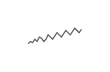
\begin{tikzpicture}[x=0.08em, y=0.08em, line width=0.4pt]
                \draw[FooterGray] (0,3) -- (1,4) -- (2,3.5) -- (3,5) -- (4,4) -- (5,6) -- (6,5.5) -- (7,4) -- (8,5) -- (9,7) -- (10,6) -- (11,5) -- (12,6.5) -- (13,8) -- (14,7) -- (15,6) -- (16,7.5) -- (17,9) -- (18,8) -- (19,7) -- (20,8.5) -- (21,10) -- (22,9) -- (23,8) -- (24,9.5);
            \end{tikzpicture}%
        }%
        \hskip0.5cm%
    }%
    \vskip6pt%
}

%=============================================================================
% PACKAGES
%=============================================================================
\usepackage[utf8]{inputenc}
\DeclareUnicodeCharacter{03B1}{\ensuremath{\alpha}}
\usepackage[T1]{fontenc}
\usepackage{amsmath, amssymb, amsthm}
\usepackage{mathtools}
\usepackage{bm}
\usepackage{tikz}
\usetikzlibrary{arrows.meta, positioning, shapes, calc, decorations.pathreplacing, shadings}
\usepackage{booktabs}
\usepackage{multirow}
\usepackage{array}
\usepackage{graphicx}
\usepackage{animate}
\usepackage{hyperref}
\usepackage{colortbl}
\usepackage{listings}
\lstset{language=Python, basicstyle=\ttfamily\scriptsize, keywordstyle=\color{MainBlue}\bfseries,
  commentstyle=\color{Forest}, stringstyle=\color{Crimson}, breaklines=true,
  frame=none, backgroundcolor=\color{VeryLightGray}, xleftmargin=2mm}
\hypersetup{colorlinks=true, linkcolor=MainBlue, urlcolor=MainBlue}
\graphicspath{{../../logos/}{../../charts/}{../../photos/}}
\usepackage{xcolor}
\hfuzz=2pt  % Suppress tiny overfull warnings (<2pt)
\vfuzz=2pt  % Suppress tiny vertical overfull warnings (<2pt)
% \mathrm in the sans-serif family of the slides (beamer resets \mathrm to the serif family at \begin{document};
% this hook runs after beamer's, so WN, Var, RMSE, ... in formulas match the surrounding text)
% Bold vectors and matrices in the same sans-serif family: \mathbf{A} in sans bold (beamer's own \mathbf came out in
% medium weight), and the bold upright Greek capitals of \boldsymbol / \bm (\bSigma, \bPhi, \boldsymbol{\Theta}) in
% cmss bold: bm.sty fixes its "boldoperators" font when it is loaded (serif cmbx), before beamer switches the
% operators to cmss, so it is reset here.
\AtBeginDocument{%
  \SetMathAlphabet{\mathrm}{normal}{\encodingdefault}{\sfdefault}{\mddefault}{n}%
  \SetMathAlphabet{\mathrm}{bold}{\encodingdefault}{\sfdefault}{bx}{n}%
  \SetMathAlphabet{\mathbf}{normal}{\encodingdefault}{\sfdefault}{bx}{n}%
  \SetMathAlphabet{\mathbf}{bold}{\encodingdefault}{\sfdefault}{bx}{n}%
  \SetSymbolFont{boldoperators}{normal}{OT1}{cmss}{bx}{n}%
  \SetSymbolFont{boldoperators}{bold}{OT1}{cmss}{bx}{n}}

%=============================================================================
% QUANTLET COMMANDS
%   \quantlet{<displayed name>}{<url>}       (generic, compatible with the older TSA decks)
%   \tsaquantlet{Ch_05}{TSA_ch5_garch}       -> https://github.com/danpele/Time-Series-Analysis/tree/main/Quantlets/Ch_05/TSA_ch5_garch
%   \qlurl{<folder>} is defined per chapter by the generator (Quantlets/Ch_NN/<folder>)
%=============================================================================
\newcommand{\tsarepo}{https://github.com/danpele/Time-Series-Analysis}
\newcommand{\tsaqlbase}{https://github.com/danpele/Time-Series-Analysis/tree/main/Quantlets}
\newcommand{\quantlet}[2]{%
    \hfill\href{#2}{%
        \raisebox{-0.15em}{
\includegraphics[height=0.7em]{ql_logo.png}}%
        \textcolor{MainBlue}{\tiny\ #1}%
    }%
}
\newcommand{\tsaquantlet}[2]{\quantlet{\detokenize{#2}}{\tsaqlbase/#1/#2}}

%=============================================================================
% NOTEBOOKS (Google Colab)
%   \colaburl{notebooks/EN/chapter5_seminar_notebook.ipynb} -> the Colab link of a file in the TSA repo
%   \nb: the chapter notebook (each seminar deck redefines it with \renewcommand)
%=============================================================================
\newcommand{\colaburl}[1]{https://colab.research.google.com/github/danpele/Time-Series-Analysis/blob/main/#1}
\newcommand{\nb}{https://colab.research.google.com/github/danpele/Time-Series-Analysis/tree/main/notebooks/EN}
\newcommand{\nbname}{notebooks/EN}

%=============================================================================
% SLIDE HELPERS (used by the generators; the same as in MFM)
%=============================================================================
% local font size for list bodies (the preamble forces \normalsize)
\newcommand{\itemsize}[1]{\setbeamertemplate{itemize/enumerate body begin}{#1}\setbeamertemplate{itemize/enumerate subbody begin}{#1}}
\newcommand{\intitle}[1]{{\hypersetup{urlcolor=white}#1}}   % white links inside coloured title bars
\newcommand{\imgcap}[1]{{\scriptsize #1}\\[0.5mm]}          % caption under a photo
\newcommand{\imgcredit}[2]{{\tiny\color{FooterGray}\href{#1}{#2}}}   % image credit: source URL, author/licence
\newcommand{\aiprompt}[1]{{\ttfamily\color{MainBlue}#1}}     % a prompt to an AI assistant

%=============================================================================
% SEMINARS: student version by default; the instructor wrapper *_solutions.tex sets \solutionstrue
%=============================================================================
\makeatletter\@ifundefined{ifsolutions}{\expandafter\newif\csname ifsolutions\endcsname}{}\makeatother
\newcommand{\solonly}[1]{\ifsolutions #1\fi}
\newcommand{\propsub}{\ifsolutions\else\framesubtitle{\ifdefined\tsalang Rezolvarea se discută la seminar\else Solution discussed in class\fi}\fi}

%=============================================================================
% APPENDIX AND CHAPTER LINKS (latex/appendix_links.py writes the calls; it also re-declares these
% macros before \begin{document}, so the decks compile with or without this preamble block)
%=============================================================================
\providecommand{\tsaapplink}[3]{\hypertarget{#2}{}\hyperlink{#1}{\beamergotobutton{#3}}}
\providecommand{\tsaappback}[2]{\begin{tikzpicture}[remember picture,overlay]\node[anchor=south east] at ([xshift=-3mm,yshift=7mm]current page.south east){\hyperlink{#1}{\beamerreturnbutton{#2}}};\end{tikzpicture}}
\providecommand{\tsachlink}[2]{\href{#1}{#2}}
\providecommand{\tsachlinkt}[2]{\href{#1}{\usebeamercolor[fg]{frametitle}#2}}

%=============================================================================
% QUANTINAR COMMAND: link către un curs Quantinar (subiecte avansate)
%=============================================================================
\newcommand{\quantinar}[2]{%
    \href{#2}{%
        \raisebox{-0.15em}{
\includegraphics[height=0.8em]{qr_logo.png}}%
        \textcolor{MainBlue}{\scriptsize\ #1}%
    }%
}

%=============================================================================
% CUSTOM TITLE PAGE
%=============================================================================
\defbeamertemplate*{title page}{hybrid}[1][]
{
    \vspace{0.2cm}
    % Logos row - top header (with clickable links)
    \begin{center}
        \href{https://www.ase.ro}{
\includegraphics[height=1.0cm]{ase_logo.png}}\hspace{0.3cm}%
        \href{https://theida.net}{
\includegraphics[height=1.0cm]{ida_logo.png}}\hspace{0.3cm}%
        \href{https://blockchain-research-center.com}{
\includegraphics[height=1.0cm]{brc_logo.png}}\hspace{0.3cm}%
        \href{https://www.ai4efin.ase.ro}{
\includegraphics[height=1.0cm]{ai4efin_logo.png}}\hspace{0.3cm}%
        \href{https://ipe.ro/new}{
\includegraphics[height=1.0cm]{acad_logo.png}}\hspace{0.3cm}%
        \href{https://www.digital-finance-msca.com}{
\includegraphics[height=1.0cm]{msca_logo.png}}%
    \end{center}

    \vspace{0.6cm}

    % Main title with Q logos on sides (with clickable links)
    \begin{center}
        \begin{minipage}{0.1\textwidth}
            \centering
            \href{https://quantlet.com}{
\includegraphics[height=1.1cm]{ql_logo.png}}
        \end{minipage}%
        \begin{minipage}{0.78\textwidth}
            \centering
            {\LARGE\bfseries\usebeamercolor[fg]{title}\inserttitle}

            \vspace{0.3cm}

            {\usebeamerfont{subtitle}\usebeamercolor[fg]{title}\insertsubtitle}
        \end{minipage}%
        \begin{minipage}{0.1\textwidth}
            \centering
            \href{https://quantinar.com}{
\includegraphics[height=1.1cm]{qr_logo.png}}
        \end{minipage}
    \end{center}

    \vspace{0.6cm}

    % Authors (left aligned)
    \hspace{0.5cm}{\usebeamerfont{author}\insertauthor}

    \vspace{0.3cm}

    % Institute/Affiliations (left aligned)
    \hspace{0.5cm}\begin{minipage}[t]{0.9\textwidth}
        \raggedright\small\insertinstitute
    \end{minipage}
}

%=============================================================================
% THEOREM ENVIRONMENTS
%=============================================================================
\theoremstyle{definition}
\setbeamertemplate{theorems}[numbered]
\ifdefined\tsalang
\newtheorem{defn}{Definiție}
\newtheorem{thm}{Teoremă}
\newtheorem{prop}{Propoziție}
\newtheorem{rmk}{Observație}
\else
\newtheorem{defn}{Definition}
\newtheorem{thm}{Theorem}
\newtheorem{prop}{Proposition}
\newtheorem{rmk}{Remark}
\fi

%=============================================================================
% CENTRED MINIPAGE (no extra vertical space)
%=============================================================================
\newenvironment{cminipage}[1]{%
    \par\noindent\hfill\begin{minipage}{#1}\ignorespaces
}{%
    \end{minipage}\hfill\null\par
}

%=============================================================================
% CUSTOM COMMANDS
%=============================================================================
\newcommand{\E}{\mathbb{E}}
\newcommand{\Var}{\text{Var}}
\newcommand{\Cov}{\text{Cov}}
\newcommand{\Corr}{\text{Corr}}
\newcommand{\R}{\mathbb{R}}
\newcommand{\N}{\mathbb{N}}
\newcommand{\Z}{\mathbb{Z}}
\newcommand{\B}{\mathbf{B}}
\newcommand{\imark}{\textcolor{MainBlue}{\textbullet}}
\newcommand{\RMSE}{\text{RMSE}}
\newcommand{\MAE}{\text{MAE}}
\newcommand{\MAPE}{\text{MAPE}}

% Boldface vector/matrix commands (VAR, VECM, state space; also used by the older TSA decks)
\newcommand{\bY}{\mathbf{Y}}
\newcommand{\bX}{\mathbf{X}}
\newcommand{\bA}{\mathbf{A}}
\newcommand{\bB}{\mathbf{B}}
\newcommand{\bepsilon}{\boldsymbol{\varepsilon}}
\newcommand{\bSigma}{\boldsymbol{\Sigma}}
\newcommand{\bPhi}{\boldsymbol{\Phi}}
\newcommand{\bGamma}{\boldsymbol{\Gamma}}
\newcommand{\bPi}{\boldsymbol{\Pi}}
\newcommand{\bc}{\mathbf{c}}
\newcommand{\balpha}{\boldsymbol{\alpha}}
\newcommand{\bbeta}{\boldsymbol{\beta}}
\newcommand{\bvarepsilon}{\boldsymbol{\varepsilon}}

% Legacy seminar marks (older TSA seminar decks)
\newcommand{\correct}{\textcolor{Forest}{\checkmark}}
\newcommand{\incorrect}{\textcolor{Crimson}{\texttimes}}
 se definește
%   \newcommand{\coursename}{Time Series Analysis}      (EN)
%   \newcommand{\coursename}{Serii de timp}       (RO)  și  \def\tsalang{ro}
% Fișierele .tex se află în EN/Courses, EN/Seminars, RO/Cursuri, RO/Seminarii (două niveluri sub rădăcină).
% Deck-urile sînt generate de latex/build_chapterN.py / build_seminarN.py (vezi latex/tsa_build.py).

\documentclass[9pt, aspectratio=169, t]{beamer}
\providecommand{\coursename}{Time Series Analysis}

% Ensure content fits on slides
\setbeamersize{text margin left=8mm, text margin right=8mm}
% Smaller institute font (title page)
\setbeamerfont{institute}{size=\footnotesize}

%=============================================================================
% THEME AND STYLE CONFIGURATION
%=============================================================================
\usetheme{default}
% Using default theme for clean header/footer control

% Color Palette (matching Redispatch PDF)
\definecolor{MainBlue}{RGB}{26, 58, 110}
\definecolor{AccentBlue}{RGB}{26, 58, 110}
\definecolor{IDAred}{RGB}{205, 0, 0}
\definecolor{DarkGray}{RGB}{51, 51, 51}
\definecolor{MediumGray}{RGB}{128, 128, 128}
\definecolor{LightGray}{RGB}{248, 248, 248}
\definecolor{VeryLightGray}{RGB}{235, 235, 235}
\definecolor{KeynoteGray}{RGB}{218, 218, 218}
\definecolor{SectionGray}{RGB}{120, 120, 120}
\definecolor{FooterGray}{RGB}{100, 100, 100}
\definecolor{Crimson}{RGB}{220, 53, 69}
\definecolor{Forest}{RGB}{46, 125, 50}
\definecolor{Amber}{RGB}{181, 133, 63}
\definecolor{Orange}{RGB}{230, 126, 34}
\definecolor{Purple}{RGB}{142, 68, 173}

% Gradient background (exact Keynote 315° gradient: white to RGB 218,218,218)
\setbeamertemplate{background}{%
    \begin{tikzpicture}[remember picture, overlay]
        \shade[shading=axis, shading angle=315,
        top color=white, bottom color=KeynoteGray]
        (current page.south west) rectangle (current page.north east);
    \end{tikzpicture}%
}
% Fallback solid color for compatibility
\setbeamercolor{background canvas}{bg=}

\setbeamercolor{palette primary}{bg=MainBlue, fg=white}
\setbeamercolor{palette secondary}{bg=MainBlue!85, fg=white}
\setbeamercolor{palette tertiary}{bg=MainBlue!70, fg=white}
\setbeamercolor{structure}{fg=MainBlue}
\setbeamercolor{title}{fg=IDAred}
\setbeamercolor{frametitle}{fg=IDAred, bg=}
\setbeamercolor{block title}{bg=MainBlue, fg=white}
\setbeamercolor{block body}{bg=VeryLightGray, fg=DarkGray}
\setbeamercolor{block title alerted}{bg=Crimson, fg=white}
\setbeamercolor{block body alerted}{bg=Crimson!8, fg=DarkGray}
\setbeamercolor{block title example}{bg=Forest, fg=white}
\setbeamercolor{block body example}{bg=Forest!8, fg=DarkGray}
\setbeamercolor{item}{fg=MainBlue}

% Footer colors (override Madrid theme blue)
\setbeamercolor{author in head/foot}{fg=FooterGray, bg=}
\setbeamercolor{title in head/foot}{fg=FooterGray, bg=}
\setbeamercolor{date in head/foot}{fg=FooterGray, bg=}
\setbeamercolor{section in head/foot}{fg=FooterGray, bg=}
\setbeamercolor{subsection in head/foot}{fg=FooterGray, bg=}

% Bullet styles (apply everywhere including blocks)
\setbeamertemplate{itemize item}{\color{MainBlue}$\boxdot$}
\setbeamertemplate{itemize subitem}{\color{MainBlue}$\blacktriangleright$}
\setbeamertemplate{itemize subsubitem}{\color{MainBlue}\tiny$\bullet$}
\setbeamertemplate{itemize/enumerate body begin}{\normalsize}
\setbeamertemplate{itemize/enumerate subbody begin}{\normalsize}

% Item spacing - compact style
\setlength{\leftmargini}{10pt}       % Level 1: minimal indent
\setlength{\leftmarginii}{10pt}      % Level 2: minimal additional indent
% Compact list spacing (zero extra space before/after lists in blocks)
\makeatletter
\def\@listi{\leftmargin\leftmargini \topsep 0pt \parsep 0pt \itemsep 0pt}
\def\@listii{\leftmargin\leftmarginii \topsep 0pt \parsep 0pt \itemsep 0pt}
\makeatother

\setbeamertemplate{navigation symbols}{}

%=============================================================================
% CUSTOM HEADLINE
%=============================================================================
\setbeamertemplate{headline}{%
    \vskip10pt%
    \hbox to \paperwidth{%
        \hskip0.5cm%
        {\small\color{FooterGray}\renewcommand{\hyperlink}[2]{##2}\insertsectionhead}%
        \hfill%
        \textcolor{FooterGray}{\small\insertframenumber}%
        \hskip0.5cm%
    }%
    \vskip4pt%
    {\color{FooterGray}\hrule height 0.4pt}%
}

%=============================================================================
% CUSTOM FOOTER
%=============================================================================
\usepackage{fontawesome5}

\setbeamertemplate{footline}{%
    {\color{FooterGray}\hrule height 0.4pt}%
    \vskip4pt%
    \hbox to \paperwidth{%
        \hskip0.5cm%
        \textcolor{FooterGray}{\small\coursename}%
        \hfill%
        \raisebox{-0.1em}{%
            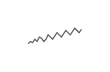
\begin{tikzpicture}[x=0.08em, y=0.08em, line width=0.4pt]
                \draw[FooterGray] (0,3) -- (1,4) -- (2,3.5) -- (3,5) -- (4,4) -- (5,6) -- (6,5.5) -- (7,4) -- (8,5) -- (9,7) -- (10,6) -- (11,5) -- (12,6.5) -- (13,8) -- (14,7) -- (15,6) -- (16,7.5) -- (17,9) -- (18,8) -- (19,7) -- (20,8.5) -- (21,10) -- (22,9) -- (23,8) -- (24,9.5);
            \end{tikzpicture}%
        }%
        \hskip0.5cm%
    }%
    \vskip6pt%
}

%=============================================================================
% PACKAGES
%=============================================================================
\usepackage[utf8]{inputenc}
\DeclareUnicodeCharacter{03B1}{\ensuremath{\alpha}}
\usepackage[T1]{fontenc}
\usepackage{amsmath, amssymb, amsthm}
\usepackage{mathtools}
\usepackage{bm}
\usepackage{tikz}
\usetikzlibrary{arrows.meta, positioning, shapes, calc, decorations.pathreplacing, shadings}
\usepackage{booktabs}
\usepackage{multirow}
\usepackage{array}
\usepackage{graphicx}
\usepackage{animate}
\usepackage{hyperref}
\usepackage{colortbl}
\usepackage{listings}
\lstset{language=Python, basicstyle=\ttfamily\scriptsize, keywordstyle=\color{MainBlue}\bfseries,
  commentstyle=\color{Forest}, stringstyle=\color{Crimson}, breaklines=true,
  frame=none, backgroundcolor=\color{VeryLightGray}, xleftmargin=2mm}
\hypersetup{colorlinks=true, linkcolor=MainBlue, urlcolor=MainBlue}
\graphicspath{{../../logos/}{../../charts/}{../../photos/}}
\usepackage{xcolor}
\hfuzz=2pt  % Suppress tiny overfull warnings (<2pt)
\vfuzz=2pt  % Suppress tiny vertical overfull warnings (<2pt)
% \mathrm in the sans-serif family of the slides (beamer resets \mathrm to the serif family at \begin{document};
% this hook runs after beamer's, so WN, Var, RMSE, ... in formulas match the surrounding text)
% Bold vectors and matrices in the same sans-serif family: \mathbf{A} in sans bold (beamer's own \mathbf came out in
% medium weight), and the bold upright Greek capitals of \boldsymbol / \bm (\bSigma, \bPhi, \boldsymbol{\Theta}) in
% cmss bold: bm.sty fixes its "boldoperators" font when it is loaded (serif cmbx), before beamer switches the
% operators to cmss, so it is reset here.
\AtBeginDocument{%
  \SetMathAlphabet{\mathrm}{normal}{\encodingdefault}{\sfdefault}{\mddefault}{n}%
  \SetMathAlphabet{\mathrm}{bold}{\encodingdefault}{\sfdefault}{bx}{n}%
  \SetMathAlphabet{\mathbf}{normal}{\encodingdefault}{\sfdefault}{bx}{n}%
  \SetMathAlphabet{\mathbf}{bold}{\encodingdefault}{\sfdefault}{bx}{n}%
  \SetSymbolFont{boldoperators}{normal}{OT1}{cmss}{bx}{n}%
  \SetSymbolFont{boldoperators}{bold}{OT1}{cmss}{bx}{n}}

%=============================================================================
% QUANTLET COMMANDS
%   \quantlet{<displayed name>}{<url>}       (generic, compatible with the older TSA decks)
%   \tsaquantlet{Ch_05}{TSA_ch5_garch}       -> https://github.com/danpele/Time-Series-Analysis/tree/main/Quantlets/Ch_05/TSA_ch5_garch
%   \qlurl{<folder>} is defined per chapter by the generator (Quantlets/Ch_NN/<folder>)
%=============================================================================
\newcommand{\tsarepo}{https://github.com/danpele/Time-Series-Analysis}
\newcommand{\tsaqlbase}{https://github.com/danpele/Time-Series-Analysis/tree/main/Quantlets}
\newcommand{\quantlet}[2]{%
    \hfill\href{#2}{%
        \raisebox{-0.15em}{
\includegraphics[height=0.7em]{ql_logo.png}}%
        \textcolor{MainBlue}{\tiny\ #1}%
    }%
}
\newcommand{\tsaquantlet}[2]{\quantlet{\detokenize{#2}}{\tsaqlbase/#1/#2}}

%=============================================================================
% NOTEBOOKS (Google Colab)
%   \colaburl{notebooks/EN/chapter5_seminar_notebook.ipynb} -> the Colab link of a file in the TSA repo
%   \nb: the chapter notebook (each seminar deck redefines it with \renewcommand)
%=============================================================================
\newcommand{\colaburl}[1]{https://colab.research.google.com/github/danpele/Time-Series-Analysis/blob/main/#1}
\newcommand{\nb}{https://colab.research.google.com/github/danpele/Time-Series-Analysis/tree/main/notebooks/EN}
\newcommand{\nbname}{notebooks/EN}

%=============================================================================
% SLIDE HELPERS (used by the generators; the same as in MFM)
%=============================================================================
% local font size for list bodies (the preamble forces \normalsize)
\newcommand{\itemsize}[1]{\setbeamertemplate{itemize/enumerate body begin}{#1}\setbeamertemplate{itemize/enumerate subbody begin}{#1}}
\newcommand{\intitle}[1]{{\hypersetup{urlcolor=white}#1}}   % white links inside coloured title bars
\newcommand{\imgcap}[1]{{\scriptsize #1}\\[0.5mm]}          % caption under a photo
\newcommand{\imgcredit}[2]{{\tiny\color{FooterGray}\href{#1}{#2}}}   % image credit: source URL, author/licence
\newcommand{\aiprompt}[1]{{\ttfamily\color{MainBlue}#1}}     % a prompt to an AI assistant

%=============================================================================
% SEMINARS: student version by default; the instructor wrapper *_solutions.tex sets \solutionstrue
%=============================================================================
\makeatletter\@ifundefined{ifsolutions}{\expandafter\newif\csname ifsolutions\endcsname}{}\makeatother
\newcommand{\solonly}[1]{\ifsolutions #1\fi}
\newcommand{\propsub}{\ifsolutions\else\framesubtitle{\ifdefined\tsalang Rezolvarea se discută la seminar\else Solution discussed in class\fi}\fi}

%=============================================================================
% APPENDIX AND CHAPTER LINKS (latex/appendix_links.py writes the calls; it also re-declares these
% macros before \begin{document}, so the decks compile with or without this preamble block)
%=============================================================================
\providecommand{\tsaapplink}[3]{\hypertarget{#2}{}\hyperlink{#1}{\beamergotobutton{#3}}}
\providecommand{\tsaappback}[2]{\begin{tikzpicture}[remember picture,overlay]\node[anchor=south east] at ([xshift=-3mm,yshift=7mm]current page.south east){\hyperlink{#1}{\beamerreturnbutton{#2}}};\end{tikzpicture}}
\providecommand{\tsachlink}[2]{\href{#1}{#2}}
\providecommand{\tsachlinkt}[2]{\href{#1}{\usebeamercolor[fg]{frametitle}#2}}

%=============================================================================
% QUANTINAR COMMAND: link către un curs Quantinar (subiecte avansate)
%=============================================================================
\newcommand{\quantinar}[2]{%
    \href{#2}{%
        \raisebox{-0.15em}{
\includegraphics[height=0.8em]{qr_logo.png}}%
        \textcolor{MainBlue}{\scriptsize\ #1}%
    }%
}

%=============================================================================
% CUSTOM TITLE PAGE
%=============================================================================
\defbeamertemplate*{title page}{hybrid}[1][]
{
    \vspace{0.2cm}
    % Logos row - top header (with clickable links)
    \begin{center}
        \href{https://www.ase.ro}{
\includegraphics[height=1.0cm]{ase_logo.png}}\hspace{0.3cm}%
        \href{https://theida.net}{
\includegraphics[height=1.0cm]{ida_logo.png}}\hspace{0.3cm}%
        \href{https://blockchain-research-center.com}{
\includegraphics[height=1.0cm]{brc_logo.png}}\hspace{0.3cm}%
        \href{https://www.ai4efin.ase.ro}{
\includegraphics[height=1.0cm]{ai4efin_logo.png}}\hspace{0.3cm}%
        \href{https://ipe.ro/new}{
\includegraphics[height=1.0cm]{acad_logo.png}}\hspace{0.3cm}%
        \href{https://www.digital-finance-msca.com}{
\includegraphics[height=1.0cm]{msca_logo.png}}%
    \end{center}

    \vspace{0.6cm}

    % Main title with Q logos on sides (with clickable links)
    \begin{center}
        \begin{minipage}{0.1\textwidth}
            \centering
            \href{https://quantlet.com}{
\includegraphics[height=1.1cm]{ql_logo.png}}
        \end{minipage}%
        \begin{minipage}{0.78\textwidth}
            \centering
            {\LARGE\bfseries\usebeamercolor[fg]{title}\inserttitle}

            \vspace{0.3cm}

            {\usebeamerfont{subtitle}\usebeamercolor[fg]{title}\insertsubtitle}
        \end{minipage}%
        \begin{minipage}{0.1\textwidth}
            \centering
            \href{https://quantinar.com}{
\includegraphics[height=1.1cm]{qr_logo.png}}
        \end{minipage}
    \end{center}

    \vspace{0.6cm}

    % Authors (left aligned)
    \hspace{0.5cm}{\usebeamerfont{author}\insertauthor}

    \vspace{0.3cm}

    % Institute/Affiliations (left aligned)
    \hspace{0.5cm}\begin{minipage}[t]{0.9\textwidth}
        \raggedright\small\insertinstitute
    \end{minipage}
}

%=============================================================================
% THEOREM ENVIRONMENTS
%=============================================================================
\theoremstyle{definition}
\setbeamertemplate{theorems}[numbered]
\ifdefined\tsalang
\newtheorem{defn}{Definiție}
\newtheorem{thm}{Teoremă}
\newtheorem{prop}{Propoziție}
\newtheorem{rmk}{Observație}
\else
\newtheorem{defn}{Definition}
\newtheorem{thm}{Theorem}
\newtheorem{prop}{Proposition}
\newtheorem{rmk}{Remark}
\fi

%=============================================================================
% CENTRED MINIPAGE (no extra vertical space)
%=============================================================================
\newenvironment{cminipage}[1]{%
    \par\noindent\hfill\begin{minipage}{#1}\ignorespaces
}{%
    \end{minipage}\hfill\null\par
}

%=============================================================================
% CUSTOM COMMANDS
%=============================================================================
\newcommand{\E}{\mathbb{E}}
\newcommand{\Var}{\text{Var}}
\newcommand{\Cov}{\text{Cov}}
\newcommand{\Corr}{\text{Corr}}
\newcommand{\R}{\mathbb{R}}
\newcommand{\N}{\mathbb{N}}
\newcommand{\Z}{\mathbb{Z}}
\newcommand{\B}{\mathbf{B}}
\newcommand{\imark}{\textcolor{MainBlue}{\textbullet}}
\newcommand{\RMSE}{\text{RMSE}}
\newcommand{\MAE}{\text{MAE}}
\newcommand{\MAPE}{\text{MAPE}}

% Boldface vector/matrix commands (VAR, VECM, state space; also used by the older TSA decks)
\newcommand{\bY}{\mathbf{Y}}
\newcommand{\bX}{\mathbf{X}}
\newcommand{\bA}{\mathbf{A}}
\newcommand{\bB}{\mathbf{B}}
\newcommand{\bepsilon}{\boldsymbol{\varepsilon}}
\newcommand{\bSigma}{\boldsymbol{\Sigma}}
\newcommand{\bPhi}{\boldsymbol{\Phi}}
\newcommand{\bGamma}{\boldsymbol{\Gamma}}
\newcommand{\bPi}{\boldsymbol{\Pi}}
\newcommand{\bc}{\mathbf{c}}
\newcommand{\balpha}{\boldsymbol{\alpha}}
\newcommand{\bbeta}{\boldsymbol{\beta}}
\newcommand{\bvarepsilon}{\boldsymbol{\varepsilon}}

% Legacy seminar marks (older TSA seminar decks)
\newcommand{\correct}{\textcolor{Forest}{\checkmark}}
\newcommand{\incorrect}{\textcolor{Crimson}{\texttimes}}
 se definește
%   \newcommand{\coursename}{Time Series Analysis}      (EN)
%   \newcommand{\coursename}{Serii de timp}       (RO)  și  \def\tsalang{ro}
% Fișierele .tex se află în EN/Courses, EN/Seminars, RO/Cursuri, RO/Seminarii (două niveluri sub rădăcină).
% Deck-urile sînt generate de latex/build_chapterN.py / build_seminarN.py (vezi latex/tsa_build.py).

\documentclass[9pt, aspectratio=169, t]{beamer}
\providecommand{\coursename}{Time Series Analysis}

% Ensure content fits on slides
\setbeamersize{text margin left=8mm, text margin right=8mm}
% Smaller institute font (title page)
\setbeamerfont{institute}{size=\footnotesize}

%=============================================================================
% THEME AND STYLE CONFIGURATION
%=============================================================================
\usetheme{default}
% Using default theme for clean header/footer control

% Color Palette (matching Redispatch PDF)
\definecolor{MainBlue}{RGB}{26, 58, 110}
\definecolor{AccentBlue}{RGB}{26, 58, 110}
\definecolor{IDAred}{RGB}{205, 0, 0}
\definecolor{DarkGray}{RGB}{51, 51, 51}
\definecolor{MediumGray}{RGB}{128, 128, 128}
\definecolor{LightGray}{RGB}{248, 248, 248}
\definecolor{VeryLightGray}{RGB}{235, 235, 235}
\definecolor{KeynoteGray}{RGB}{218, 218, 218}
\definecolor{SectionGray}{RGB}{120, 120, 120}
\definecolor{FooterGray}{RGB}{100, 100, 100}
\definecolor{Crimson}{RGB}{220, 53, 69}
\definecolor{Forest}{RGB}{46, 125, 50}
\definecolor{Amber}{RGB}{181, 133, 63}
\definecolor{Orange}{RGB}{230, 126, 34}
\definecolor{Purple}{RGB}{142, 68, 173}

% Gradient background (exact Keynote 315° gradient: white to RGB 218,218,218)
\setbeamertemplate{background}{%
    \begin{tikzpicture}[remember picture, overlay]
        \shade[shading=axis, shading angle=315,
        top color=white, bottom color=KeynoteGray]
        (current page.south west) rectangle (current page.north east);
    \end{tikzpicture}%
}
% Fallback solid color for compatibility
\setbeamercolor{background canvas}{bg=}

\setbeamercolor{palette primary}{bg=MainBlue, fg=white}
\setbeamercolor{palette secondary}{bg=MainBlue!85, fg=white}
\setbeamercolor{palette tertiary}{bg=MainBlue!70, fg=white}
\setbeamercolor{structure}{fg=MainBlue}
\setbeamercolor{title}{fg=IDAred}
\setbeamercolor{frametitle}{fg=IDAred, bg=}
\setbeamercolor{block title}{bg=MainBlue, fg=white}
\setbeamercolor{block body}{bg=VeryLightGray, fg=DarkGray}
\setbeamercolor{block title alerted}{bg=Crimson, fg=white}
\setbeamercolor{block body alerted}{bg=Crimson!8, fg=DarkGray}
\setbeamercolor{block title example}{bg=Forest, fg=white}
\setbeamercolor{block body example}{bg=Forest!8, fg=DarkGray}
\setbeamercolor{item}{fg=MainBlue}

% Footer colors (override Madrid theme blue)
\setbeamercolor{author in head/foot}{fg=FooterGray, bg=}
\setbeamercolor{title in head/foot}{fg=FooterGray, bg=}
\setbeamercolor{date in head/foot}{fg=FooterGray, bg=}
\setbeamercolor{section in head/foot}{fg=FooterGray, bg=}
\setbeamercolor{subsection in head/foot}{fg=FooterGray, bg=}

% Bullet styles (apply everywhere including blocks)
\setbeamertemplate{itemize item}{\color{MainBlue}$\boxdot$}
\setbeamertemplate{itemize subitem}{\color{MainBlue}$\blacktriangleright$}
\setbeamertemplate{itemize subsubitem}{\color{MainBlue}\tiny$\bullet$}
\setbeamertemplate{itemize/enumerate body begin}{\normalsize}
\setbeamertemplate{itemize/enumerate subbody begin}{\normalsize}

% Item spacing - compact style
\setlength{\leftmargini}{10pt}       % Level 1: minimal indent
\setlength{\leftmarginii}{10pt}      % Level 2: minimal additional indent
% Compact list spacing (zero extra space before/after lists in blocks)
\makeatletter
\def\@listi{\leftmargin\leftmargini \topsep 0pt \parsep 0pt \itemsep 0pt}
\def\@listii{\leftmargin\leftmarginii \topsep 0pt \parsep 0pt \itemsep 0pt}
\makeatother

\setbeamertemplate{navigation symbols}{}

%=============================================================================
% CUSTOM HEADLINE
%=============================================================================
\setbeamertemplate{headline}{%
    \vskip10pt%
    \hbox to \paperwidth{%
        \hskip0.5cm%
        {\small\color{FooterGray}\renewcommand{\hyperlink}[2]{##2}\insertsectionhead}%
        \hfill%
        \textcolor{FooterGray}{\small\insertframenumber}%
        \hskip0.5cm%
    }%
    \vskip4pt%
    {\color{FooterGray}\hrule height 0.4pt}%
}

%=============================================================================
% CUSTOM FOOTER
%=============================================================================
\usepackage{fontawesome5}

\setbeamertemplate{footline}{%
    {\color{FooterGray}\hrule height 0.4pt}%
    \vskip4pt%
    \hbox to \paperwidth{%
        \hskip0.5cm%
        \textcolor{FooterGray}{\small\coursename}%
        \hfill%
        \raisebox{-0.1em}{%
            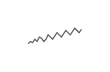
\begin{tikzpicture}[x=0.08em, y=0.08em, line width=0.4pt]
                \draw[FooterGray] (0,3) -- (1,4) -- (2,3.5) -- (3,5) -- (4,4) -- (5,6) -- (6,5.5) -- (7,4) -- (8,5) -- (9,7) -- (10,6) -- (11,5) -- (12,6.5) -- (13,8) -- (14,7) -- (15,6) -- (16,7.5) -- (17,9) -- (18,8) -- (19,7) -- (20,8.5) -- (21,10) -- (22,9) -- (23,8) -- (24,9.5);
            \end{tikzpicture}%
        }%
        \hskip0.5cm%
    }%
    \vskip6pt%
}

%=============================================================================
% PACKAGES
%=============================================================================
\usepackage[utf8]{inputenc}
\DeclareUnicodeCharacter{03B1}{\ensuremath{\alpha}}
\usepackage[T1]{fontenc}
\usepackage{amsmath, amssymb, amsthm}
\usepackage{mathtools}
\usepackage{bm}
\usepackage{tikz}
\usetikzlibrary{arrows.meta, positioning, shapes, calc, decorations.pathreplacing, shadings}
\usepackage{booktabs}
\usepackage{multirow}
\usepackage{array}
\usepackage{graphicx}
\usepackage{animate}
\usepackage{hyperref}
\usepackage{colortbl}
\usepackage{listings}
\lstset{language=Python, basicstyle=\ttfamily\scriptsize, keywordstyle=\color{MainBlue}\bfseries,
  commentstyle=\color{Forest}, stringstyle=\color{Crimson}, breaklines=true,
  frame=none, backgroundcolor=\color{VeryLightGray}, xleftmargin=2mm}
\hypersetup{colorlinks=true, linkcolor=MainBlue, urlcolor=MainBlue}
\graphicspath{{../../logos/}{../../charts/}{../../photos/}}
\usepackage{xcolor}
\hfuzz=2pt  % Suppress tiny overfull warnings (<2pt)
\vfuzz=2pt  % Suppress tiny vertical overfull warnings (<2pt)
% \mathrm in the sans-serif family of the slides (beamer resets \mathrm to the serif family at \begin{document};
% this hook runs after beamer's, so WN, Var, RMSE, ... in formulas match the surrounding text)
% Bold vectors and matrices in the same sans-serif family: \mathbf{A} in sans bold (beamer's own \mathbf came out in
% medium weight), and the bold upright Greek capitals of \boldsymbol / \bm (\bSigma, \bPhi, \boldsymbol{\Theta}) in
% cmss bold: bm.sty fixes its "boldoperators" font when it is loaded (serif cmbx), before beamer switches the
% operators to cmss, so it is reset here.
\AtBeginDocument{%
  \SetMathAlphabet{\mathrm}{normal}{\encodingdefault}{\sfdefault}{\mddefault}{n}%
  \SetMathAlphabet{\mathrm}{bold}{\encodingdefault}{\sfdefault}{bx}{n}%
  \SetMathAlphabet{\mathbf}{normal}{\encodingdefault}{\sfdefault}{bx}{n}%
  \SetMathAlphabet{\mathbf}{bold}{\encodingdefault}{\sfdefault}{bx}{n}%
  \SetSymbolFont{boldoperators}{normal}{OT1}{cmss}{bx}{n}%
  \SetSymbolFont{boldoperators}{bold}{OT1}{cmss}{bx}{n}}

%=============================================================================
% QUANTLET COMMANDS
%   \quantlet{<displayed name>}{<url>}       (generic, compatible with the older TSA decks)
%   \tsaquantlet{Ch_05}{TSA_ch5_garch}       -> https://github.com/danpele/Time-Series-Analysis/tree/main/Quantlets/Ch_05/TSA_ch5_garch
%   \qlurl{<folder>} is defined per chapter by the generator (Quantlets/Ch_NN/<folder>)
%=============================================================================
\newcommand{\tsarepo}{https://github.com/danpele/Time-Series-Analysis}
\newcommand{\tsaqlbase}{https://github.com/danpele/Time-Series-Analysis/tree/main/Quantlets}
\newcommand{\quantlet}[2]{%
    \hfill\href{#2}{%
        \raisebox{-0.15em}{
\includegraphics[height=0.7em]{ql_logo.png}}%
        \textcolor{MainBlue}{\tiny\ #1}%
    }%
}
\newcommand{\tsaquantlet}[2]{\quantlet{\detokenize{#2}}{\tsaqlbase/#1/#2}}

%=============================================================================
% NOTEBOOKS (Google Colab)
%   \colaburl{notebooks/EN/chapter5_seminar_notebook.ipynb} -> the Colab link of a file in the TSA repo
%   \nb: the chapter notebook (each seminar deck redefines it with \renewcommand)
%=============================================================================
\newcommand{\colaburl}[1]{https://colab.research.google.com/github/danpele/Time-Series-Analysis/blob/main/#1}
\newcommand{\nb}{https://colab.research.google.com/github/danpele/Time-Series-Analysis/tree/main/notebooks/EN}
\newcommand{\nbname}{notebooks/EN}

%=============================================================================
% SLIDE HELPERS (used by the generators; the same as in MFM)
%=============================================================================
% local font size for list bodies (the preamble forces \normalsize)
\newcommand{\itemsize}[1]{\setbeamertemplate{itemize/enumerate body begin}{#1}\setbeamertemplate{itemize/enumerate subbody begin}{#1}}
\newcommand{\intitle}[1]{{\hypersetup{urlcolor=white}#1}}   % white links inside coloured title bars
\newcommand{\imgcap}[1]{{\scriptsize #1}\\[0.5mm]}          % caption under a photo
\newcommand{\imgcredit}[2]{{\tiny\color{FooterGray}\href{#1}{#2}}}   % image credit: source URL, author/licence
\newcommand{\aiprompt}[1]{{\ttfamily\color{MainBlue}#1}}     % a prompt to an AI assistant

%=============================================================================
% SEMINARS: student version by default; the instructor wrapper *_solutions.tex sets \solutionstrue
%=============================================================================
\makeatletter\@ifundefined{ifsolutions}{\expandafter\newif\csname ifsolutions\endcsname}{}\makeatother
\newcommand{\solonly}[1]{\ifsolutions #1\fi}
\newcommand{\propsub}{\ifsolutions\else\framesubtitle{\ifdefined\tsalang Rezolvarea se discută la seminar\else Solution discussed in class\fi}\fi}

%=============================================================================
% APPENDIX AND CHAPTER LINKS (latex/appendix_links.py writes the calls; it also re-declares these
% macros before \begin{document}, so the decks compile with or without this preamble block)
%=============================================================================
\providecommand{\tsaapplink}[3]{\hypertarget{#2}{}\hyperlink{#1}{\beamergotobutton{#3}}}
\providecommand{\tsaappback}[2]{\begin{tikzpicture}[remember picture,overlay]\node[anchor=south east] at ([xshift=-3mm,yshift=7mm]current page.south east){\hyperlink{#1}{\beamerreturnbutton{#2}}};\end{tikzpicture}}
\providecommand{\tsachlink}[2]{\href{#1}{#2}}
\providecommand{\tsachlinkt}[2]{\href{#1}{\usebeamercolor[fg]{frametitle}#2}}

%=============================================================================
% QUANTINAR COMMAND: link către un curs Quantinar (subiecte avansate)
%=============================================================================
\newcommand{\quantinar}[2]{%
    \href{#2}{%
        \raisebox{-0.15em}{
\includegraphics[height=0.8em]{qr_logo.png}}%
        \textcolor{MainBlue}{\scriptsize\ #1}%
    }%
}

%=============================================================================
% CUSTOM TITLE PAGE
%=============================================================================
\defbeamertemplate*{title page}{hybrid}[1][]
{
    \vspace{0.2cm}
    % Logos row - top header (with clickable links)
    \begin{center}
        \href{https://www.ase.ro}{
\includegraphics[height=1.0cm]{ase_logo.png}}\hspace{0.3cm}%
        \href{https://theida.net}{
\includegraphics[height=1.0cm]{ida_logo.png}}\hspace{0.3cm}%
        \href{https://blockchain-research-center.com}{
\includegraphics[height=1.0cm]{brc_logo.png}}\hspace{0.3cm}%
        \href{https://www.ai4efin.ase.ro}{
\includegraphics[height=1.0cm]{ai4efin_logo.png}}\hspace{0.3cm}%
        \href{https://ipe.ro/new}{
\includegraphics[height=1.0cm]{acad_logo.png}}\hspace{0.3cm}%
        \href{https://www.digital-finance-msca.com}{
\includegraphics[height=1.0cm]{msca_logo.png}}%
    \end{center}

    \vspace{0.6cm}

    % Main title with Q logos on sides (with clickable links)
    \begin{center}
        \begin{minipage}{0.1\textwidth}
            \centering
            \href{https://quantlet.com}{
\includegraphics[height=1.1cm]{ql_logo.png}}
        \end{minipage}%
        \begin{minipage}{0.78\textwidth}
            \centering
            {\LARGE\bfseries\usebeamercolor[fg]{title}\inserttitle}

            \vspace{0.3cm}

            {\usebeamerfont{subtitle}\usebeamercolor[fg]{title}\insertsubtitle}
        \end{minipage}%
        \begin{minipage}{0.1\textwidth}
            \centering
            \href{https://quantinar.com}{
\includegraphics[height=1.1cm]{qr_logo.png}}
        \end{minipage}
    \end{center}

    \vspace{0.6cm}

    % Authors (left aligned)
    \hspace{0.5cm}{\usebeamerfont{author}\insertauthor}

    \vspace{0.3cm}

    % Institute/Affiliations (left aligned)
    \hspace{0.5cm}\begin{minipage}[t]{0.9\textwidth}
        \raggedright\small\insertinstitute
    \end{minipage}
}

%=============================================================================
% THEOREM ENVIRONMENTS
%=============================================================================
\theoremstyle{definition}
\setbeamertemplate{theorems}[numbered]
\ifdefined\tsalang
\newtheorem{defn}{Definiție}
\newtheorem{thm}{Teoremă}
\newtheorem{prop}{Propoziție}
\newtheorem{rmk}{Observație}
\else
\newtheorem{defn}{Definition}
\newtheorem{thm}{Theorem}
\newtheorem{prop}{Proposition}
\newtheorem{rmk}{Remark}
\fi

%=============================================================================
% CENTRED MINIPAGE (no extra vertical space)
%=============================================================================
\newenvironment{cminipage}[1]{%
    \par\noindent\hfill\begin{minipage}{#1}\ignorespaces
}{%
    \end{minipage}\hfill\null\par
}

%=============================================================================
% CUSTOM COMMANDS
%=============================================================================
\newcommand{\E}{\mathbb{E}}
\newcommand{\Var}{\text{Var}}
\newcommand{\Cov}{\text{Cov}}
\newcommand{\Corr}{\text{Corr}}
\newcommand{\R}{\mathbb{R}}
\newcommand{\N}{\mathbb{N}}
\newcommand{\Z}{\mathbb{Z}}
\newcommand{\B}{\mathbf{B}}
\newcommand{\imark}{\textcolor{MainBlue}{\textbullet}}
\newcommand{\RMSE}{\text{RMSE}}
\newcommand{\MAE}{\text{MAE}}
\newcommand{\MAPE}{\text{MAPE}}

% Boldface vector/matrix commands (VAR, VECM, state space; also used by the older TSA decks)
\newcommand{\bY}{\mathbf{Y}}
\newcommand{\bX}{\mathbf{X}}
\newcommand{\bA}{\mathbf{A}}
\newcommand{\bB}{\mathbf{B}}
\newcommand{\bepsilon}{\boldsymbol{\varepsilon}}
\newcommand{\bSigma}{\boldsymbol{\Sigma}}
\newcommand{\bPhi}{\boldsymbol{\Phi}}
\newcommand{\bGamma}{\boldsymbol{\Gamma}}
\newcommand{\bPi}{\boldsymbol{\Pi}}
\newcommand{\bc}{\mathbf{c}}
\newcommand{\balpha}{\boldsymbol{\alpha}}
\newcommand{\bbeta}{\boldsymbol{\beta}}
\newcommand{\bvarepsilon}{\boldsymbol{\varepsilon}}

% Legacy seminar marks (older TSA seminar decks)
\newcommand{\correct}{\textcolor{Forest}{\checkmark}}
\newcommand{\incorrect}{\textcolor{Crimson}{\texttimes}}


\newcommand{\qlurl}[1]{https://github.com/danpele/Time-Series-Analysis/tree/main/Quantlets/Ch_15/#1}

% Clickable citations (DOIs verified via Crossref)
\newcommand{\refHP}{\href{https://doi.org/10.1007/978-3-031-13584-2}{Huang and Petukhina (2022)}}
\newcommand{\refFPP}{\href{https://otexts.com/fpp3/}{Hyndman and Athanasopoulos (2021)}}
\newcommand{\refBD}{\href{https://doi.org/10.1007/978-3-319-29854-2}{Brockwell and Davis (2016)}}
\newcommand{\refHamilton}{\href{https://doi.org/10.2307/j.ctv14jx6sm}{Hamilton (1994)}}
\newcommand{\refBJ}{\href{https://doi.org/10.1002/9781118619193}{Box, Jenkins and Reinsel (2008)}}
\newcommand{\refLB}{\href{https://doi.org/10.1093/biomet/65.2.297}{Ljung and Box (1978)}}
\newcommand{\refAkaike}{\href{https://doi.org/10.1109/TAC.1974.1100705}{Akaike (1974)}}
\newcommand{\refSchwarz}{\href{https://doi.org/10.1214/aos/1176344136}{Schwarz (1978)}}
\newcommand{\refDF}{\href{https://doi.org/10.1080/01621459.1979.10482531}{Dickey and Fuller (1979)}}
\newcommand{\refKPSS}{\href{https://doi.org/10.1016/0304-4076(92)90104-Y}{Kwiatkowski et al.\ (1992)}}
\newcommand{\refGN}{\href{https://doi.org/10.1016/0304-4076(74)90034-7}{Granger and Newbold (1974)}}
\newcommand{\refDM}{\href{https://doi.org/10.1080/07350015.1995.10524599}{Diebold and Mariano (1995)}}
\newcommand{\refHLN}{\href{https://doi.org/10.1016/S0169-2070(96)00719-4}{Harvey, Leybourne and Newbold (1997)}}
\newcommand{\refEngle}{\href{https://doi.org/10.2307/1912773}{Engle (1982)}}
\newcommand{\refBoll}{\href{https://doi.org/10.1016/0304-4076(86)90063-1}{Bollerslev (1986)}}
\newcommand{\refSims}{\href{https://doi.org/10.2307/1912017}{Sims (1980)}}
\newcommand{\refGranger}{\href{https://doi.org/10.2307/1912791}{Granger (1969)}}
\newcommand{\refEG}{\href{https://doi.org/10.2307/1913236}{Engle and Granger (1987)}}
\newcommand{\refJoh}{\href{https://doi.org/10.2307/2938278}{Johansen (1991)}}
\newcommand{\refGJ}{\href{https://doi.org/10.1111/j.1467-9892.1980.tb00297.x}{Granger and Joyeux (1980)}}
\newcommand{\refHosking}{\href{https://doi.org/10.1093/biomet/68.1.165}{Hosking (1981)}}
\newcommand{\refMfour}{\href{https://doi.org/10.1016/j.ijforecast.2019.04.014}{Makridakis, Spiliotis and Assimakopoulos (2020)}}
\newcommand{\refKalman}{\href{https://doi.org/10.1115/1.3662552}{Kalman (1960)}}
\newcommand{\refHamMS}{\href{https://doi.org/10.2307/1912559}{Hamilton (1989)}}

\title[Time Series Analysis]{Time Series Analysis}
\subtitle{Chapter 15: Review and exam preparation}
\author[D.T. Pele]{Daniel Traian PELE}
\institute{Bucharest University of Economic Studies\\
IDA Institute Digital Assets\\
Blockchain Research Center\\
AI4EFin Artificial Intelligence for Energy Finance\\
Romanian Academy, Institute for Economic Forecasting\\
MSCA Digital Finance}
\date{}

%=============================================================================
\providecommand{\tsaapplink}[3]{\hypertarget{#2}{}\hyperlink{#1}{\beamergotobutton{#3}}}  % APPLINKS-MACROS
\providecommand{\tsaappback}[2]{\begin{tikzpicture}[remember picture,overlay]\node[anchor=south east] at ([xshift=-3mm,yshift=7mm]current page.south east){\hyperlink{#1}{\beamerreturnbutton{#2}}};\end{tikzpicture}}  % APPLINKS-MACROS
\providecommand{\tsachlink}[2]{\href{#1}{#2}}  % APPLINKS-MACROS
\providecommand{\tsachlinkt}[2]{\href{#1}{\usebeamercolor[fg]{frametitle}#2}}  % APPLINKS-MACROS
\begin{document}
%=============================================================================

{
\setbeamertemplate{headline}{}
\setbeamertemplate{footline}{}
\begin{frame}[noframenumbering]
    \titlepage
\end{frame}
}
% BEGIN-ACRONYMS (generat de latex/acronyms.py; nu editati manual)
\begin{frame}{Acronyms used in this material (1/3)}
\setbeamertemplate{itemize/enumerate body begin}{\tiny}
\begin{columns}[T]
\begin{column}{0.49\textwidth}
\begin{itemize}\setlength{\itemsep}{0pt}
    \item \textbf{ACF}: Autocorrelation Function
    \item \textbf{ADF}: Augmented Dickey–Fuller (test)
    \item \textbf{AI}: Artificial Intelligence
    \item \textbf{AIC}: Akaike Information Criterion
    \item \textbf{AR}: AutoRegressive (model); in event studies: Abnormal Return
    \item \textbf{ARCH}: AutoRegressive Conditional Heteroskedasticity
    \item \textbf{ARCH-LM}: ARCH Lagrange Multiplier (test)
    \item \textbf{ARFIMA}: AutoRegressive Fractionally Integrated Moving Average (model)
    \item \textbf{ARIMA}: AutoRegressive Integrated Moving Average (model)
    \item \textbf{ARMA}: AutoRegressive Moving Average (model)
    \item \textbf{BEKK}: Baba–Engle–Kraft–Kroner (multivariate GARCH model)
    \item \textbf{BET}: Bucharest Exchange Trading (index)
    \item \textbf{BIC}: Bayesian Information Criterion
\end{itemize}
\end{column}
\begin{column}{0.49\textwidth}
\begin{itemize}\setlength{\itemsep}{0pt}
    \item \textbf{BNR}: Banca Națională a României (the National Bank of Romania)
    \item \textbf{BVB}: Bursa de Valori București (the Bucharest Stock Exchange)
    \item \textbf{CCC}: Constant Conditional Correlation (model)
    \item \textbf{DCC}: Dynamic Conditional Correlation
    \item \textbf{DHR}: Dynamic Harmonic Regression
    \item \textbf{DLOG}: Difference of the LOGarithm (EViews function)
    \item \textbf{DM}: Diebold–Mariano (test)
    \item \textbf{EC1}: Error Correction term 1
    \item \textbf{EC2}: Error Correction term 2
    \item \textbf{ECM}: Error Correction Model
    \item \textbf{ENTSO-E}: European Network of Transmission System Operators for Electricity
    \item \textbf{EODHD}: EOD Historical Data (market-data provider)
    \item \textbf{FEVD}: Forecast Error Variance Decomposition
\end{itemize}
\end{column}
\end{columns}
\end{frame}
\begin{frame}{Acronyms used in this material (2/3)}
\setbeamertemplate{itemize/enumerate body begin}{\tiny}
\begin{columns}[T]
\begin{column}{0.49\textwidth}
\begin{itemize}\setlength{\itemsep}{0pt}
    \item \textbf{FRED}: Federal Reserve Economic Data
    \item \textbf{GARCH}: Generalised AutoRegressive Conditional Heteroskedasticity
    \item \textbf{GDP}: Gross Domestic Product
    \item \textbf{GJR}: Glosten–Jagannathan–Runkle (GARCH model)
    \item \textbf{GPH}: Geweke–Porter-Hudak (estimator)
    \item \textbf{HEGY}: Hylleberg–Engle–Granger–Yoo (seasonal unit-root test)
    \item \textbf{HICP}: Harmonised Index of Consumer Prices
    \item \textbf{HLN}: Harvey–Leybourne–Newbold (small-sample correction of the DM test)
    \item \textbf{HP}: Hodrick–Prescott (filter)
    \item \textbf{IPC}: Indicele prețurilor de consum (the consumer price index (CPI))
    \item \textbf{IRF}: Impulse Response Function
    \item \textbf{KPSS}: Kwiatkowski–Phillips–Schmidt–Shin (test)
    \item \textbf{LB}: Ljung–Box (test)
\end{itemize}
\end{column}
\begin{column}{0.49\textwidth}
\begin{itemize}\setlength{\itemsep}{0pt}
    \item \textbf{LPPL}: Log-Periodic Power Law
    \item \textbf{LPPLS}: Log-Periodic Power Law Singularity (model)
    \item \textbf{LSTM}: Long Short-Term Memory (network)
    \item \textbf{MA}: Moving Average
    \item \textbf{MAE}: Mean Absolute Error
    \item \textbf{MAPE}: Mean Absolute Percentage Error
    \item \textbf{MASE}: Mean Absolute Scaled Error
    \item \textbf{NBER}: National Bureau of Economic Research
    \item \textbf{OCSB}: Osborn–Chui–Smith–Birchenhall (seasonal unit-root test)
    \item \textbf{OLS}: Ordinary Least Squares
    \item \textbf{PACF}: Partial AutoCorrelation Function
    \item \textbf{PPP}: Purchasing Power Parity
    \item \textbf{QQ}: Quantile–Quantile (plot)
\end{itemize}
\end{column}
\end{columns}
\end{frame}
\begin{frame}{Acronyms used in this material (3/3)}
\setbeamertemplate{itemize/enumerate body begin}{\tiny}
\begin{columns}[T]
\begin{column}{0.49\textwidth}
\begin{itemize}\setlength{\itemsep}{0pt}
    \item \textbf{RMSE}: Root Mean Squared Error
    \item \textbf{ROBOR}: Romanian Interbank Offer Rate
    \item \textbf{SAR}: Seasonal AutoRegressive term (EViews)
    \item \textbf{SARIMA}: Seasonal ARIMA (model)
    \item \textbf{SE}: Standard Error
    \item \textbf{SES}: Simple Exponential Smoothing
    \item \textbf{SIGMASQ}: SIGMA SQuared, the innovation variance (EViews)
    \item \textbf{US}: United States
    \item \textbf{VAR}: Vector AutoRegression
    \item \textbf{VAT}: Value Added Tax
    \item \textbf{VEC}: Vector (half-vectorised) GARCH model
    \item \textbf{VECM}: Vector Error Correction Model
\end{itemize}
\end{column}
\begin{column}{0.49\textwidth}
\end{column}
\end{columns}
\end{frame}
% END-ACRONYMS

\begin{frame}{Today's question and route}
\itemsize{\small}
\begin{columns}[T]
\begin{column}{0.58\textwidth}
\begin{itemize}
    \item \textbf{Question}: what does the whole course say about a time series, and how is it examined?
    \begin{itemize}
        \item one chapter that ties \tsachlink{https://danpele.github.io/Time-Series-Analysis/EN/Courses/chapter0_introduction.pdf}{Chapters 0}--\tsachlink{https://danpele.github.io/Time-Series-Analysis/EN/Courses/chapter14_multivariate_garch_models.pdf}{14} together
    \end{itemize}
    \item \textbf{Route}
    \begin{itemize}
        \item Part I: the course map, two recap slides per chapter, the toolbox of tests and models
        \item Part II: the Box--Jenkins method from start to finish on Romanian inflation
        \item Part III: the exam (format, grading, eight solved problems), the team project and attendance
    \end{itemize}
    \item \tsachlink{https://danpele.github.io/Time-Series-Analysis/EN/Courses/chapter11_foundation_models_time_series.pdf}{Chapters 11}--\tsachlink{https://danpele.github.io/Time-Series-Analysis/EN/Courses/chapter14_multivariate_garch_models.pdf}{14} are for self-study
\end{itemize}
\end{column}
\begin{column}{0.38\textwidth}
\centering
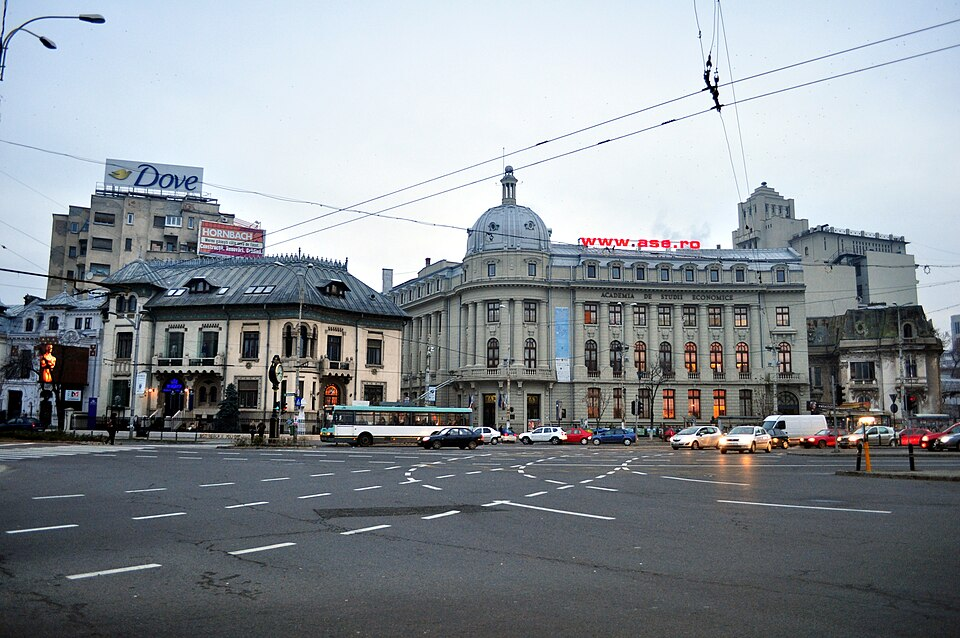
\includegraphics[height=0.40\textheight]{ch0_ase_2014.jpg}\\[1mm]
\imgcap{Bucharest University of Economic Studies}
\imgcredit{https://commons.wikimedia.org/wiki/File:Bucharest_-_Academie_de_Studii_Economice_01.jpg}{Photo: Joe Mabel (2014); CC BY 3.0; Wikimedia Commons}
\end{column}
\end{columns}
\end{frame}

\begin{frame}{Learning outcomes}
\itemsize{\small}
\begin{itemize}
    \item Place every chapter on the path from describing a series to modelling and forecasting it
    \item Recall the key formula, the key empirical fact and the most common mistake of each chapter
    \item Choose the right test or model for a given question about a time series
    \item Run the Box--Jenkins method on a real series: transform, test, identify, estimate, check, forecast
    \item Read software output (estimates, tests, correlograms) and interpret it in three to five sentences
    \item Plan the team project, its oral defence and the declaration of AI use
\end{itemize}
\end{frame}

\begin{frame}{Reading and tools}
\itemsize{\small}
\begin{itemize}
    \item Textbook: \refHP; free companion: \refFPP
    \begin{itemize}
        \item theory: \refBD; \refHamilton; the method: \refBJ
    \end{itemize}
    \item Python Quantlets of this chapter: \href{https://github.com/danpele/Time-Series-Analysis/tree/main/Quantlets/Ch_15}{Quantlets/Ch\_15}
    \begin{itemize}
        \item the Box--Jenkins case on the Romanian HICP and the output of exam problem 3
    \end{itemize}
    \item Lecture notebook, the course in one notebook: \href{\colaburl{notebooks/EN/chapter15_lecture_notebook.ipynb}}{open in Google Colab}
    \item Self-assessment: the quiz of this chapter, 20 questions drawn from all chapters
\end{itemize}
\end{frame}


%=============================================================================
\section{The course map}
%=============================================================================

\begin{frame}{The course map: \tsachlinkt{https://danpele.github.io/Time-Series-Analysis/EN/Courses/chapter0_introduction.pdf}{Chapters 0}--\tsachlinkt{https://danpele.github.io/Time-Series-Analysis/EN/Courses/chapter14_multivariate_garch_models.pdf}{14}}
\itemsize{\footnotesize}
\begin{center}
\resizebox{0.97\textwidth}{!}{%
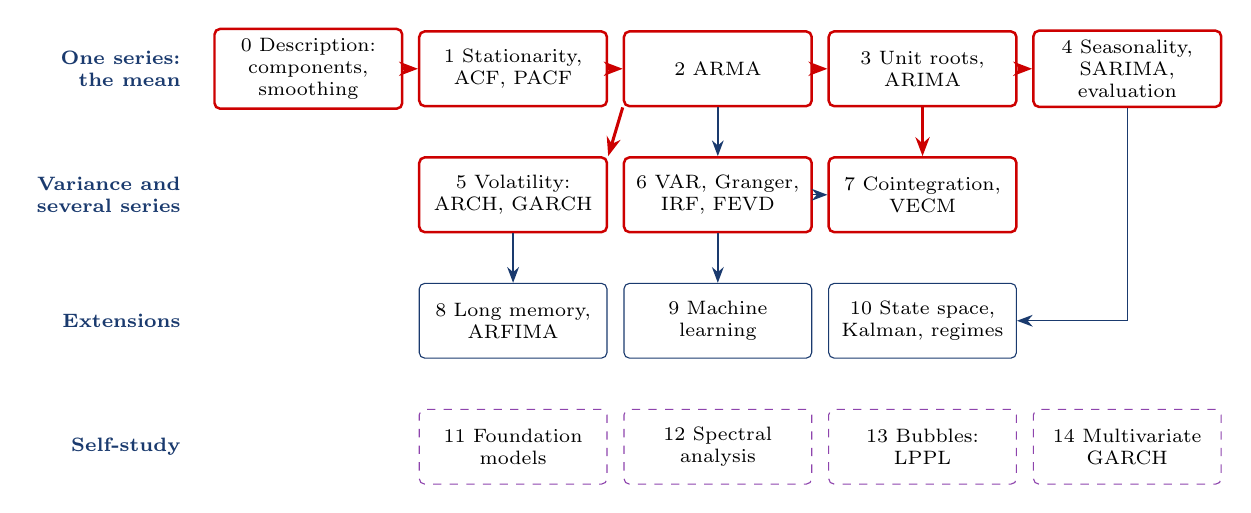
\begin{tikzpicture}[
  box/.style={draw=MainBlue, rounded corners=2pt, fill=white, font=\scriptsize, align=center, minimum height=0.95cm, text width=2.15cm},
  key/.style={box, draw=IDAred, line width=0.9pt},
  self/.style={box, dashed, draw=Purple},
  lab/.style={font=\scriptsize\bfseries, text=MainBlue, anchor=east, align=right},
  arr/.style={-{Stealth[length=2mm]}, MainBlue, line width=0.5pt},
  karr/.style={-{Stealth[length=2.4mm]}, IDAred, line width=1.1pt},
  sarr/.style={-{Stealth[length=2mm]}, Purple, dashed, line width=0.5pt}]
\node[lab] at (-0.2, 0) {One series:\\ the mean};
\node[key] (c0) at (1.3, 0) {0 Description:\\ components, smoothing};
\node[key] (c1) at (3.9, 0) {1 Stationarity,\\ ACF, PACF};
\node[key] (c2) at (6.5, 0) {2 ARMA};
\node[key] (c3) at (9.1, 0) {3 Unit roots,\\ ARIMA};
\node[key] (c4) at (11.7, 0) {4 Seasonality,\\ SARIMA, evaluation};
\node[lab] at (-0.2, -1.6) {Variance and\\ several series};
\node[key] (c5) at (3.9, -1.6) {5 Volatility:\\ ARCH, GARCH};
\node[key] (c6) at (6.5, -1.6) {6 VAR, Granger,\\ IRF, FEVD};
\node[key] (c7) at (9.1, -1.6) {7 Cointegration,\\ VECM};
\node[lab] at (-0.2, -3.2) {Extensions};
\node[box] (c8) at (3.9, -3.2) {8 Long memory,\\ ARFIMA};
\node[box] (c9) at (6.5, -3.2) {9 Machine\\ learning};
\node[box] (c10) at (9.1, -3.2) {10 State space,\\ Kalman, regimes};
\node[lab] at (-0.2, -4.8) {Self-study};
\node[self] (c11) at (3.9, -4.8) {11 Foundation\\ models};
\node[self] (c12) at (6.5, -4.8) {12 Spectral\\ analysis};
\node[self] (c13) at (9.1, -4.8) {13 Bubbles:\\ LPPL};
\node[self] (c14) at (11.7, -4.8) {14 Multivariate\\ GARCH};
\draw[karr] (c0) -- (c1); \draw[karr] (c1) -- (c2); \draw[karr] (c2) -- (c3); \draw[karr] (c3) -- (c4);
\draw[karr] (c2.south west) -- (c5.north east); \draw[karr] (c3) -- (c7); \draw[arr] (c2) -- (c6); \draw[arr] (c6) -- (c7);
\draw[arr] (c5) -- (c8); \draw[arr] (c6) -- (c9); \draw[arr] (c4.south) -- (11.7, -3.2) -- (c10.east);
\end{tikzpicture}}
\end{center}
\vspace{-0.2cm}
\begin{itemize}
    \item Red: the core of the exam, from describing one series to modelling several series together
    \item Blue: extensions (\tsachlink{https://danpele.github.io/Time-Series-Analysis/EN/Courses/chapter8_long_memory_arfima.pdf}{Chapters 8}--\tsachlink{https://danpele.github.io/Time-Series-Analysis/EN/Courses/chapter10_state_space_kalman_markov_switching.pdf}{10}); dashed: self-study (\tsachlink{https://danpele.github.io/Time-Series-Analysis/EN/Courses/chapter11_foundation_models_time_series.pdf}{Chapters 11}--\tsachlink{https://danpele.github.io/Time-Series-Analysis/EN/Courses/chapter14_multivariate_garch_models.pdf}{14}), each built on a core chapter: 11 on 9, 12 on 1 and 8, 13 on 3, 14 on 5 and 6
\end{itemize}
\end{frame}

\begin{frame}{The series of the course}
\itemsize{\small}
\begin{center}
\footnotesize
\begin{tabular}{>{\raggedright\arraybackslash}p{3.6cm}>{\raggedright\arraybackslash}p{2.6cm}>{\raggedright\arraybackslash}p{4.2cm}l}
\toprule
\textbf{Series} & \textbf{Source} & \textbf{Topic illustrated} & \textbf{Ch.} \\
\midrule
Romanian real GDP (quarterly) & Eurostat & trend, seasonality, a unit root, regimes & 0--4, 10 \\
Romanian HICP inflation (monthly) & Eurostat & persistence, seasonality, long memory & 2--4, 8 \\
ROBOR 3M, unemployment & Eurostat & a VAR for the Romanian economy & 6 \\
EUR/RON & BNR & a random walk that is hard to beat & 0, 3, 5 \\
BET, S\&P 500, DAX (daily) & EODHD & volatility clustering, spillovers & 1, 5, 6 \\
electricity load (daily, hourly) & ENTSO-E & multiple seasonality, machine learning & 4, 9 \\
Nile, sunspots, US yields and GDP & statsmodels, FRED & the classic examples of the textbooks & 1, 2, 7, 8, 10 \\
\bottomrule
\end{tabular}
\end{center}
\begin{itemize}
    \item Every number on the recap slides is the number of its chapter: same data, same window, same code
\end{itemize}
\end{frame}


%=============================================================================
\section{Chapters 0--3: description, stationarity, ARMA, ARIMA}
%=============================================================================

\begin{frame}{\tsachlinkt{https://danpele.github.io/Time-Series-Analysis/EN/Courses/chapter0_introduction.pdf}{Chapter 0}: Introduction: components and exponential smoothing (1/2)}
\itemsize{\footnotesize}
\begin{itemize}
    \item \textbf{Key formulas}
    \begin{itemize}
        \item additive $y_t = T_t + S_t + R_t$ or multiplicative $y_t = T_t S_t R_t$; the logarithm turns one into the other
        \item SES $\ell_t = \alpha y_t + (1 - \alpha)\ell_{t-1}$; MASE $=$ MAE $/$ MAE of the in-sample seasonal naive method
    \end{itemize}
    \item \textbf{Notation}
    \begin{itemize}
        \item $T_t$, $S_t$, $R_t$: the trend, the seasonal component and the remainder (the irregular part)
        \item $\ell_t$: the smoothed level at time $t$; $\alpha \in (0, 1)$: the weight of the newest observation; a large $\alpha$ follows the data closely
        \item MAE: the mean absolute error; MASE below 1: better than the seasonal naive method
    \end{itemize}
\end{itemize}
\end{frame}

\begin{frame}{\tsachlinkt{https://danpele.github.io/Time-Series-Analysis/EN/Courses/chapter0_introduction.pdf}{Chapter 0}: Introduction: components and exponential smoothing (2/2)}
\itemsize{\footnotesize}
\begin{itemize}
    \item \textbf{Empirical facts}
    \begin{itemize}
        \item Romanian GDP grew 2.3 times since 1995 (2.8\% a year); Q1 is about $\ensuremath{-}23.8\%$ and Q4 $+20.7\%$ around the trend
        \item EUR/RON: $\hat\alpha_{SES} = 1.00$, the last value is the best forecast; electricity: Holt--Winters MASE 0.51 against 0.82 for the naive method
    \end{itemize}
    \item \textbf{Common mistakes}
    \begin{itemize}
        \item judging a forecast on the data used to fit it
        \item MAPE for series that cross zero (monthly inflation); an additive model for a seasonal swing that grows with the level
    \end{itemize}
\end{itemize}
\end{frame}

\begin{frame}{\tsachlinkt{https://danpele.github.io/Time-Series-Analysis/EN/Courses/chapter1_stochastic_processes_stationarity.pdf}{Chapter 1}: Stochastic processes and stationarity (1/2)}
\itemsize{\footnotesize}
\begin{itemize}
    \item \textbf{Key formulas}
    \begin{itemize}
        \item weak stationarity: $E X_t = \mu$, $\mathrm{Cov}(X_t, X_{t+h}) = \gamma(h)$; $\hat\rho(h)$ against $\pm 1.96/\sqrt{T}$
        \item Ljung--Box $Q^*(m) = T(T + 2)\sum_{h=1}^{m}\hat\rho(h)^2/(T - h) \sim \chi^2(m)$ \refLB; random walk $\mathrm{Var}(X_t) = t\sigma^2$
    \end{itemize}
    \item \textbf{Notation}
    \begin{itemize}
        \item $\mu$: the constant mean; $\gamma(h)$: the autocovariance at lag $h$, which depends only on $h$; $\hat\rho(h)$: the sample autocorrelation; $T$: the number of observations
        \item $Q^*(m)$: the Ljung--Box statistic on the first $m$ lags; a large value (a small p-value) rejects white noise
        \item $\sigma^2$: the variance of the random-walk shocks; $\mathrm{Var}(X_t) = t\sigma^2$ grows with $t$, so a random walk is not stationary
    \end{itemize}
\end{itemize}
\end{frame}

\begin{frame}{\tsachlinkt{https://danpele.github.io/Time-Series-Analysis/EN/Courses/chapter1_stochastic_processes_stationarity.pdf}{Chapter 1}: Stochastic processes and stationarity (2/2)}
\itemsize{\footnotesize}
\begin{itemize}
    \item \textbf{Empirical facts}
    \begin{itemize}
        \item BET returns: $\hat\rho_1 = 0.11$, absolute returns $\hat\rho_1 = 0.40$ (band $\pm 0.024$): uncorrelated is not independent
        \item Romanian GDP: Box--Cox $\hat\lambda = 0.02$, the logarithm; one difference too many gives $\hat\rho_1 = \ensuremath{-}0.54$
    \end{itemize}
    \item \textbf{Common mistakes}
    \begin{itemize}
        \item reading one bar outside the band as a signal (one in twenty is outside by chance)
        \item differencing a series that is already stationary
    \end{itemize}
\end{itemize}
\end{frame}

\begin{frame}{\tsachlinkt{https://danpele.github.io/Time-Series-Analysis/EN/Courses/chapter2_arma_models.pdf}{Chapter 2}: ARMA models (1/2)}
\itemsize{\footnotesize}
\begin{itemize}
    \item \textbf{Key formulas}
    \begin{itemize}
        \item $\phi(L)(X_t - \mu) = \theta(L)\varepsilon_t$; AR(1) $\rho(h) = \phi^h$; MA(1) $\rho(1) = \theta/(1 + \theta^2)$
        \item AIC $= -2\ln L + 2k$ \refAkaike, BIC $= -2\ln L + k\ln T$ \refSchwarz; residual check $Q^*(m) \sim \chi^2(m - p - q)$
    \end{itemize}
    \item \textbf{Notation}
    \begin{itemize}
        \item $L$: the lag operator, $LX_t = X_{t-1}$; $\phi(L)$, $\theta(L)$: the AR and MA polynomials of orders $p$ and $q$; $\varepsilon_t$: white noise
        \item $\ln L$: the maximised log-likelihood; $k$: the number of estimated parameters; a smaller AIC or BIC is better
        \item BIC penalises parameters more than AIC, since $\ln T > 2$ for $T \ge 8$
    \end{itemize}
\end{itemize}
\end{frame}

\begin{frame}{\tsachlinkt{https://danpele.github.io/Time-Series-Analysis/EN/Courses/chapter2_arma_models.pdf}{Chapter 2}: ARMA models (2/2)}
\itemsize{\footnotesize}
\begin{itemize}
    \item \textbf{Empirical facts}
    \begin{itemize}
        \item annual growth of Romanian GDP: MA(3) by BIC, a product of overlapping quarters; residual Ljung--Box $p = 0.37$
        \item Romanian inflation: AR(2) with $\hat\phi_1 + \hat\phi_2 = 0.976$, close to a unit root; sunspots: an AR(2) cycle of 10.6 years
    \end{itemize}
    \item \textbf{Common mistakes}
    \begin{itemize}
        \item reading the AR order from the ACF (it is the PACF that cuts off for an AR)
        \item Ljung--Box on residuals with $m$ instead of $m - p - q$ degrees of freedom; a common factor in $\phi(L)$ and $\theta(L)$
    \end{itemize}
\end{itemize}
\end{frame}

\begin{frame}{\tsachlinkt{https://danpele.github.io/Time-Series-Analysis/EN/Courses/chapter3_unit_roots_arima_models.pdf}{Chapter 3}: Unit roots and ARIMA models (1/2)}
\itemsize{\footnotesize}
\begin{itemize}
    \item \textbf{Key formulas}
    \begin{itemize}
        \item ADF: $\Delta y_t = c + bt + \gamma y_{t-1} + \sum_j\delta_j\Delta y_{t-j} + \varepsilon_t$, $H_0$: $\gamma = 0$ \refDF; KPSS: $H_0$ stationarity \refKPSS
        \item ARIMA$(p,d,q)$: $\phi(L)(1 - L)^d y_t = c + \theta(L)\varepsilon_t$; forecast variance grows with $h$ when $d \ge 1$
    \end{itemize}
    \item \textbf{Notation}
    \begin{itemize}
        \item $\Delta y_t = y_t - y_{t-1}$; $c$: the constant; $bt$: the deterministic trend; $\gamma = 0$ means a unit root
        \item $\delta_j$: the coefficients of the lagged differences, which remove the autocorrelation of the errors
        \item $d$: the number of differences needed for stationarity; $(1 - L)^d$: the difference of order $d$; $h$: the forecast horizon
    \end{itemize}
\end{itemize}
\end{frame}

\begin{frame}{\tsachlinkt{https://danpele.github.io/Time-Series-Analysis/EN/Courses/chapter3_unit_roots_arima_models.pdf}{Chapter 3}: Unit roots and ARIMA models (2/2)}
\itemsize{\footnotesize}
\begin{itemize}
    \item \textbf{Empirical facts}
    \begin{itemize}
        \item log Romanian GDP: $\tau = \ensuremath{-}2.31$ ($p = 0.43$, 5\% critical value $\ensuremath{-}3.45$); growth: $\tau = \ensuremath{-}10.77$; ARIMA(0,1,0) with drift 0.81\% a quarter
        \item two independent random walks: a significant $t$ in 90\% of regressions \refGN; ADF power only 12.5\% for $\phi = 0.95$, $T = 100$
    \end{itemize}
    \item \textbf{Common mistakes}
    \begin{itemize}
        \item Student or Normal critical values for the ADF statistic
        \item reading a non-rejection as proof of a unit root; a regression in levels of $I(1)$ series without a cointegration test
    \end{itemize}
\end{itemize}
\end{frame}

\begin{frame}{Recap: \tsachlinkt{https://danpele.github.io/Time-Series-Analysis/EN/Courses/chapter0_introduction.pdf}{Chapters 0}--\tsachlinkt{https://danpele.github.io/Time-Series-Analysis/EN/Courses/chapter3_unit_roots_arima_models.pdf}{3}}
\itemsize{\small}
\begin{itemize}
    \item Plot first, then transform: logarithm for a growing swing, differences for a stochastic trend
    \item ACF and PACF identify an ARMA; AIC and BIC choose; Ljung--Box on residuals checks
    \item ADF and KPSS together decide $d$; Dickey--Fuller critical values, never Student ones
\end{itemize}
\end{frame}


%=============================================================================
\section{Chapters 4--7: seasonality, volatility, VAR, VECM}
%=============================================================================

\begin{frame}{\tsachlinkt{https://danpele.github.io/Time-Series-Analysis/EN/Courses/chapter4_seasonality_forecasting.pdf}{Chapter 4}: Seasonality and forecasting (1/2)}
\itemsize{\footnotesize}
\begin{itemize}
    \item \textbf{Key formulas}
    \begin{itemize}
        \item SARIMA $\phi(L)\Phi(L^s)(1 - L)^d(1 - L^s)^D y_t = \theta(L)\Theta(L^s)\varepsilon_t$; airline $(0,1,1)(0,1,1)_s$
        \item Diebold--Mariano $\bar d/\sqrt{\hat V/n}$, $d_t = L(e_{1t}) - L(e_{2t})$ \refDM, with the HLN correction \refHLN
    \end{itemize}
    \item \textbf{Notation}
    \begin{itemize}
        \item $s$: the season length (12 for monthly data); $\Phi(L^s)$, $\Theta(L^s)$: the seasonal AR and MA polynomials; $D$: the number of seasonal differences $(1 - L^s)$
        \item $e_{1t}$, $e_{2t}$: the errors of the two forecasts; $L(\cdot)$: the loss, e.g.\ the square; $d_t$: the loss differential; $\bar d$: its mean; $\hat V$: its estimated long-run variance; $n$: the number of forecasts
        \item under equal accuracy DM is approximately $N(0, 1)$: $|\mathrm{DM}| > 1.96$ rejects at 5\%
    \end{itemize}
\end{itemize}
\end{frame}

\begin{frame}{\tsachlinkt{https://danpele.github.io/Time-Series-Analysis/EN/Courses/chapter4_seasonality_forecasting.pdf}{Chapter 4}: Seasonality and forecasting (2/2)}
\itemsize{\footnotesize}
\begin{itemize}
    \item \textbf{Empirical facts}
    \begin{itemize}
        \item airline passengers: MAPE 8.5\% for the airline model against 15.5\% for the seasonal naive method
        \item Orthodox Easter raises Romanian food sales by about 5.9\%; daily load: DHR MASE 0.89 against 1.28 (seasonal naive)
    \end{itemize}
    \item \textbf{Common mistakes}
    \begin{itemize}
        \item comparing AICc of models with different $d$ or $D$
        \item judging forecasts at a single origin; seasonally adjusted data in a SARIMA forecast of raw data
    \end{itemize}
\end{itemize}
\end{frame}

\begin{frame}{\tsachlinkt{https://danpele.github.io/Time-Series-Analysis/EN/Courses/chapter5_conditional_volatility_garch.pdf}{Chapter 5}: Conditional volatility: ARCH and GARCH (1/2)}
\itemsize{\footnotesize}
\begin{itemize}
    \item \textbf{Key formulas}
    \begin{itemize}
        \item GARCH(1,1) $\sigma_t^2 = \omega + \alpha\varepsilon_{t-1}^2 + \beta\sigma_{t-1}^2$ \refEngle, \refBoll; $\bar\sigma^2 = \omega/(1 - \alpha - \beta)$, $h_{1/2} = \ln 0.5/\ln(\alpha + \beta)$
        \item ARCH-LM $= nR^2 \sim \chi^2(q)$; VaR 1\% $= -(\mu + \sigma_{t+1}q_{0.01}(z))$
    \end{itemize}
    \item \textbf{Notation}
    \begin{itemize}
        \item $\sigma_t^2$: the conditional variance; $\varepsilon_{t-1}$: yesterday's shock; $\omega > 0$; $\alpha \ge 0$: the reaction to shocks; $\beta \ge 0$: the persistence
        \item $\bar\sigma^2$: the long-run variance, defined only if $\alpha + \beta < 1$; $h_{1/2}$: the half-life of a volatility shock
        \item ARCH-LM: $R^2$ of the regression of $\varepsilon_t^2$ on $q$ of its lags, $n$ observations; $q_{0.01}(z)$: the 1\% quantile of the standardised innovations $z_t$
    \end{itemize}
\end{itemize}
\end{frame}

\begin{frame}{\tsachlinkt{https://danpele.github.io/Time-Series-Analysis/EN/Courses/chapter5_conditional_volatility_garch.pdf}{Chapter 5}: Conditional volatility: ARCH and GARCH (2/2)}
\itemsize{\footnotesize}
\begin{itemize}
    \item \textbf{Empirical facts}
    \begin{itemize}
        \item GARCH(1,1)-$t$: $\alpha + \beta = 0.995$ for the S\&P 500 (half-life 131 days), $0.991$ for the BET (74 days)
        \item S\&P 500: GJR $\hat\gamma = 0.21$ ($t = 10.0$); kurtosis 13.7 for returns, 5.0 for standardised residuals
    \end{itemize}
    \item \textbf{Common mistakes}
    \begin{itemize}
        \item the half-life written as $1/(1 - \alpha - \beta)$; a long-run variance reported when $\alpha + \beta \ge 1$
        \item ``VaR 99\%'' or a negative VaR: the course writes VaR 1\%, a positive loss
    \end{itemize}
\end{itemize}
\end{frame}

\begin{frame}{\tsachlinkt{https://danpele.github.io/Time-Series-Analysis/EN/Courses/chapter6_var_models_granger_causality.pdf}{Chapter 6}: VAR models and Granger causality (1/2)}
\itemsize{\footnotesize}
\begin{itemize}
    \item \textbf{Key formulas}
    \begin{itemize}
        \item VAR$(p)$: $\bY_t = \bc + \bA_1\bY_{t-1} + \dots + \bA_p\bY_{t-p} + \bepsilon_t$ \refSims; stable if all eigenvalues of the companion matrix are inside the unit circle
        \item Granger $F = [(RSS_R - RSS_U)/p]\,/\,[RSS_U/(T - Kp - 1)]$ \refGranger; IRF and FEVD with a Cholesky ordering
    \end{itemize}
    \item \textbf{Notation}
    \begin{itemize}
        \item $\bY_t$: the vector of the $K$ variables; $\bc$: the constants; $\bA_i$: the $K \times K$ coefficient matrices of lag $i$; $\bepsilon_t$: the vector of shocks
        \item the companion matrix writes the VAR($p$) as a VAR(1) of dimension $Kp$
        \item $RSS_R$, $RSS_U$: the residual sums of squares without and with the lags of the tested variable; $p$: the number of restrictions
    \end{itemize}
\end{itemize}
\end{frame}

\begin{frame}{\tsachlinkt{https://danpele.github.io/Time-Series-Analysis/EN/Courses/chapter6_var_models_granger_causality.pdf}{Chapter 6}: VAR models and Granger causality (2/2)}
\itemsize{\footnotesize}
\begin{itemize}
    \item \textbf{Empirical facts}
    \begin{itemize}
        \item Romanian VAR(2) of growth, inflation and ROBOR 3M: growth Granger-causes ROBOR, $F = 7.26$, $p =$ 0.001
        \item spillovers among the S\&P 500, DAX and BET: 26.4\% on average, 57.5\% on 17 March 2020
    \end{itemize}
    \item \textbf{Common mistakes}
    \begin{itemize}
        \item reading Granger causality as causality (it is extra predictability)
        \item IRFs reported without the ordering behind them; too many lags for a short sample
    \end{itemize}
\end{itemize}
\end{frame}

\begin{frame}{\tsachlinkt{https://danpele.github.io/Time-Series-Analysis/EN/Courses/chapter7_cointegration_vecm.pdf}{Chapter 7}: Cointegration and VECM (1/2)}
\itemsize{\footnotesize}
\begin{itemize}
    \item \textbf{Key formulas}
    \begin{itemize}
        \item Engle--Granger: OLS in levels, then ADF on residuals with MacKinnon critical values \refEG; ECM half-life $\ln 0.5/\ln(1 + \gamma)$
        \item VECM $\Delta\mathbf y_t = \alpha\beta^\top\mathbf y_{t-1} + \sum_i\Gamma_i\Delta\mathbf y_{t-i} + \mathbf u_t$; trace $-T\sum_{i>r}\ln(1 - \hat\lambda_i)$ \refJoh
    \end{itemize}
    \item \textbf{Notation}
    \begin{itemize}
        \item ECM: $\gamma < 0$ is the speed of adjustment towards equilibrium
        \item $\beta$: the cointegrating vectors (the equilibrium relations); $\alpha$: the adjustment coefficients; $\Gamma_i$: the short-run dynamics; $\mathbf u_t$: the shocks
        \item $\hat\lambda_i$: the estimated eigenvalues, in decreasing order; $r$: the tested cointegration rank; a trace above its critical value rejects rank $r$
    \end{itemize}
\end{itemize}
\end{frame}

\begin{frame}{\tsachlinkt{https://danpele.github.io/Time-Series-Analysis/EN/Courses/chapter7_cointegration_vecm.pdf}{Chapter 7}: Cointegration and VECM (2/2)}
\itemsize{\footnotesize}
\begin{itemize}
    \item \textbf{Empirical facts}
    \begin{itemize}
        \item US yields at 1, 5 and 10 years: trace 54.6 $>$ 29.8 for $r = 0$, 3.12 $<$ 3.84 for $r \le 2$: rank 2; long-rate ECM half-life 20.8 months
        \item PPP for the leu: ADF $p = 0.24$ on the real exchange rate, not stationary; pairs trading on the BVB: Sharpe 0.15 gross, 0.05 net
    \end{itemize}
    \item \textbf{Common mistakes}
    \begin{itemize}
        \item Dickey--Fuller critical values for Engle--Granger residuals (they must be more negative)
        \item a VAR in differences for cointegrated series (it omits the error correction term)
    \end{itemize}
\end{itemize}
\end{frame}

\begin{frame}{Recap: \tsachlinkt{https://danpele.github.io/Time-Series-Analysis/EN/Courses/chapter4_seasonality_forecasting.pdf}{Chapters 4}--\tsachlinkt{https://danpele.github.io/Time-Series-Analysis/EN/Courses/chapter7_cointegration_vecm.pdf}{7}}
\itemsize{\small}
\begin{itemize}
    \item Seasonality: $\Delta_s$ or Fourier terms; calendar effects as regressors; evaluation with rolling origins, MASE and DM
    \item Volatility: ARCH-LM, then GARCH(1,1)-$t$; persistence close to 1; VaR 1\% with the right quantile
    \item Several series: VAR for stationary data, VECM for cointegrated $I(1)$ data; Granger is predictability
\end{itemize}
\end{frame}


%=============================================================================
\section{Chapters 8--10: long memory, machine learning, state space}
%=============================================================================

\begin{frame}{\tsachlinkt{https://danpele.github.io/Time-Series-Analysis/EN/Courses/chapter8_long_memory_arfima.pdf}{Chapter 8}: Long memory and ARFIMA (1/2)}
\itemsize{\footnotesize}
\begin{itemize}
    \item \textbf{Key formulas}
    \begin{itemize}
        \item $(1 - L)^d$ with $\pi_k = \pi_{k-1}(k - 1 - d)/k$ \refGJ, \refHosking; $\rho(k) \sim Ck^{2d-1}$; $H = d + 1/2$
        \item stationary for $d < 1/2$, mean-reverting for $d < 1$; GPH and local Whittle use the lowest $m$ frequencies
    \end{itemize}
    \item \textbf{Notation}
    \begin{itemize}
        \item $d$: the order of fractional integration; $\pi_k$: the weight of lag $k$ in the expansion of $(1 - L)^d$
        \item $C > 0$: a constant; $\rho(k) \sim Ck^{2d-1}$: the ACF decays hyperbolically, not exponentially
        \item $H$: the Hurst exponent, above 0.5 for long memory; $m$: the number of low frequencies used by GPH and local Whittle
    \end{itemize}
\end{itemize}
\end{frame}

\begin{frame}{\tsachlinkt{https://danpele.github.io/Time-Series-Analysis/EN/Courses/chapter8_long_memory_arfima.pdf}{Chapter 8}: Long memory and ARFIMA (2/2)}
\itemsize{\footnotesize}
\begin{itemize}
    \item \textbf{Empirical facts}
    \begin{itemize}
        \item Romanian monthly inflation: ARFIMA(0,$d$,0) with $\hat d = 0.31$ (SE 0.05) beats ARMA by AIC and BIC
        \item S\&P 500: $H$ (R/S) 0.53 for returns, 0.86 for $|r_t|$; the Nile: $\hat d = 0.40$, but $\ensuremath{-}0.17$ after the break of 1898
    \end{itemize}
    \item \textbf{Common mistakes}
    \begin{itemize}
        \item a break or a regime change read as long memory
        \item one bandwidth $m$ only; long memory in returns confused with long memory in volatility
    \end{itemize}
\end{itemize}
\end{frame}

\begin{frame}{\tsachlinkt{https://danpele.github.io/Time-Series-Analysis/EN/Courses/chapter9_machine_learning_time_series.pdf}{Chapter 9}: Machine learning for time series (1/2)}
\itemsize{\footnotesize}
\begin{itemize}
    \item \textbf{Key formulas}
    \begin{itemize}
        \item direct forecast $\hat y_{T+h} = \hat f_h(y_T, \dots, y_{T-p+1}, \mathbf z_{T+h})$; ridge $+\lambda\sum\beta_j^2$, lasso $+\lambda\sum|\beta_j|$
        \item bias--variance $E(y_0 - \hat f)^2 = \text{bias}^2 + \mathrm{Var}(\hat f) + \sigma^2$; walk-forward validation only
    \end{itemize}
    \item \textbf{Notation}
    \begin{itemize}
        \item $\hat f_h$: the estimated function for horizon $h$; $p$: the number of lags used; $\mathbf z_{T+h}$: known regressors, e.g.\ the calendar
        \item $\lambda \ge 0$: the strength of the penalty; $\beta_j$: the coefficients; ridge shrinks them, lasso sets some exactly to 0
        \item $y_0$: a new observation; $\sigma^2$: the noise variance, which no model can remove
    \end{itemize}
\end{itemize}
\end{frame}

\begin{frame}{\tsachlinkt{https://danpele.github.io/Time-Series-Analysis/EN/Courses/chapter9_machine_learning_time_series.pdf}{Chapter 9}: Machine learning for time series (2/2)}
\itemsize{\footnotesize}
\begin{itemize}
    \item \textbf{Empirical facts}
    \begin{itemize}
        \item S\&P 500, the same model: $R^2 = 0.37$ with random $k$-fold, $\ensuremath{-}0.39$ walk-forward: leakage
        \item sign of returns: majority class 54.4\%, boosting 52.5\%; daily load: ridge MASE 0.90, LSTM 1.16 \refMfour
    \end{itemize}
    \item \textbf{Common mistakes}
    \begin{itemize}
        \item random cross-validation and scaling on the whole sample (look-ahead)
        \item trees on trending levels (they cannot extrapolate); no simple benchmark in the comparison
    \end{itemize}
\end{itemize}
\end{frame}

\begin{frame}{\tsachlinkt{https://danpele.github.io/Time-Series-Analysis/EN/Courses/chapter10_state_space_kalman_markov_switching.pdf}{Chapter 10}: State space models, Kalman filter and Markov switching (1/2)}
\itemsize{\footnotesize}
\begin{itemize}
    \item \textbf{Key formulas}
    \begin{itemize}
        \item $y_t = Z\alpha_t + \varepsilon_t$, $\alpha_{t+1} = T\alpha_t + R\eta_t$; $K_t = P_tZ'F_t^{-1}$, $a_{t|t} = a_t + K_tv_t$ \refKalman
        \item Markov switching: durations $1/(1 - p_{ii})$, ergodic $\pi_1 = (1 - p_{22})/(2 - p_{11} - p_{22})$ \refHamMS
    \end{itemize}
    \item \textbf{Notation}
    \begin{itemize}
        \item $\alpha_t$: the hidden state (e.g.\ the level); $Z$, $T$, $R$: known system matrices; $\varepsilon_t$, $\eta_t$: the measurement and state noise
        \item $a_t$, $P_t$: the predicted state and its variance; $v_t = y_t - Za_t$: the prediction error, with variance $F_t$; $K_t$: the Kalman gain, the weight of the surprise
        \item $p_{ii}$: the probability of staying in regime $i$; $\pi_1$: the long-run share of regime 1
    \end{itemize}
\end{itemize}
\end{frame}

\begin{frame}{\tsachlinkt{https://danpele.github.io/Time-Series-Analysis/EN/Courses/chapter10_state_space_kalman_markov_switching.pdf}{Chapter 10}: State space models, Kalman filter and Markov switching (2/2)}
\itemsize{\footnotesize}
\begin{itemize}
    \item \textbf{Empirical facts}
    \begin{itemize}
        \item the Nile: $\hat q = 0.097$, steady-state gain $\bar K = 0.267$, the weight of exponential smoothing
        \item US GDP: the regimes match the NBER dates in 90\% of quarters; Romanian GDP: stable regime 15.2 quarters, volatile 11.2
    \end{itemize}
    \item \textbf{Common mistakes}
    \begin{itemize}
        \item smoothed probabilities used as if known in real time
        \item durations written as $p_{ii}/(1 - p_{ii})$; the last value of the HP gap read as a real-time estimate
    \end{itemize}
\end{itemize}
\end{frame}

\begin{frame}{Recap: \tsachlinkt{https://danpele.github.io/Time-Series-Analysis/EN/Courses/chapter8_long_memory_arfima.pdf}{Chapters 8}--\tsachlinkt{https://danpele.github.io/Time-Series-Analysis/EN/Courses/chapter10_state_space_kalman_markov_switching.pdf}{10}}
\itemsize{\small}
\begin{itemize}
    \item Long memory: hyperbolic ACF, $d$ between 0 and 1/2; check breaks and regimes before believing it
    \item Machine learning: the same supervised table, walk-forward validation, simple benchmarks
    \item State space: the Kalman filter for hidden levels and trends; Markov switching for regimes
\end{itemize}
\end{frame}


%=============================================================================
\section{Chapters 11--14: self-study}
%=============================================================================

\begin{frame}{\tsachlinkt{https://danpele.github.io/Time-Series-Analysis/EN/Courses/chapter11_foundation_models_time_series.pdf}{Chapter 11}: Foundation models for time series (self-study)}
\itemsize{\footnotesize}
\begin{itemize}
    \item \textbf{Key ideas}
    \begin{itemize}
        \item transformers pre-trained on many series: tokenisation and patching of the values
        \item Chronos, TimesFM, Moirai, Lag-Llama: zero-shot forecasts and fine-tuning
        \item a fair comparison: the same test sample, MASE, probabilistic scores, simple benchmarks
    \end{itemize}
    \item \textbf{Link with the core of the course}
    \begin{itemize}
        \item a global model of many series (\tsachlink{https://danpele.github.io/Time-Series-Analysis/EN/Courses/chapter9_machine_learning_time_series.pdf}{Chapter 9}); judged like any forecast (\tsachlink{https://danpele.github.io/Time-Series-Analysis/EN/Courses/chapter4_seasonality_forecasting.pdf}{Chapter 4})
    \end{itemize}
    \item \tsachlink{https://danpele.github.io/Time-Series-Analysis/EN/Courses/chapter11_foundation_models_time_series.pdf}{Chapters 11}--\tsachlink{https://danpele.github.io/Time-Series-Analysis/EN/Courses/chapter14_multivariate_garch_models.pdf}{14} are for self-study (not examined unless the instructor decides otherwise)
\end{itemize}
\end{frame}

\begin{frame}{\tsachlinkt{https://danpele.github.io/Time-Series-Analysis/EN/Courses/chapter12_spectral_analysis.pdf}{Chapter 12}: Spectral analysis (self-study)}
\itemsize{\footnotesize}
\begin{itemize}
    \item \textbf{Key ideas}
    \begin{itemize}
        \item the Fourier transform, the periodogram $I(\lambda_j)$ and the spectral density
        \item smoothed periodograms (Welch), filters (Hodrick--Prescott) and business cycles
        \item coherence between two series; wavelets as a time--frequency tool
    \end{itemize}
    \item \textbf{Link with the core of the course}
    \begin{itemize}
        \item the same information as the ACF, by frequency (\tsachlink{https://danpele.github.io/Time-Series-Analysis/EN/Courses/chapter1_stochastic_processes_stationarity.pdf}{Chapter 1}); the spectral pole of long memory (\tsachlink{https://danpele.github.io/Time-Series-Analysis/EN/Courses/chapter8_long_memory_arfima.pdf}{Chapter 8})
    \end{itemize}
    \item \tsachlink{https://danpele.github.io/Time-Series-Analysis/EN/Courses/chapter11_foundation_models_time_series.pdf}{Chapters 11}--\tsachlink{https://danpele.github.io/Time-Series-Analysis/EN/Courses/chapter14_multivariate_garch_models.pdf}{14} are for self-study (not examined unless the instructor decides otherwise)
\end{itemize}
\end{frame}

\begin{frame}{\tsachlinkt{https://danpele.github.io/Time-Series-Analysis/EN/Courses/chapter13_bubbles_lppl.pdf}{Chapter 13}: Speculative bubbles: LPPL models (self-study)}
\itemsize{\footnotesize}
\begin{itemize}
    \item \textbf{Key ideas}
    \begin{itemize}
        \item bubbles as super-exponential growth of prices
        \item the LPPLS model: power law plus log-periodic oscillations; estimation and filter conditions
        \item the LPPLS confidence indicator on historical bubbles and crashes
    \end{itemize}
    \item \textbf{Link with the core of the course}
    \begin{itemize}
        \item explosive roots, the opposite of unit roots (\tsachlink{https://danpele.github.io/Time-Series-Analysis/EN/Courses/chapter3_unit_roots_arima_models.pdf}{Chapter 3}); volatility before crashes (\tsachlink{https://danpele.github.io/Time-Series-Analysis/EN/Courses/chapter5_conditional_volatility_garch.pdf}{Chapter 5})
    \end{itemize}
    \item \tsachlink{https://danpele.github.io/Time-Series-Analysis/EN/Courses/chapter11_foundation_models_time_series.pdf}{Chapters 11}--\tsachlink{https://danpele.github.io/Time-Series-Analysis/EN/Courses/chapter14_multivariate_garch_models.pdf}{14} are for self-study (not examined unless the instructor decides otherwise)
\end{itemize}
\end{frame}

\begin{frame}{\tsachlinkt{https://danpele.github.io/Time-Series-Analysis/EN/Courses/chapter14_multivariate_garch_models.pdf}{Chapter 14}: Multivariate GARCH models (self-study)}
\itemsize{\footnotesize}
\begin{itemize}
    \item \textbf{Key ideas}
    \begin{itemize}
        \item time-varying covariances and correlations; the number of parameters grows fast
        \item VEC, BEKK, CCC and DCC; estimation of DCC in two steps
        \item dynamic correlations, portfolio variance and VaR 1\%
    \end{itemize}
    \item \textbf{Link with the core of the course}
    \begin{itemize}
        \item GARCH for each series (\tsachlink{https://danpele.github.io/Time-Series-Analysis/EN/Courses/chapter5_conditional_volatility_garch.pdf}{Chapter 5}) and the multivariate view of the VAR (\tsachlink{https://danpele.github.io/Time-Series-Analysis/EN/Courses/chapter6_var_models_granger_causality.pdf}{Chapter 6})
    \end{itemize}
    \item \tsachlink{https://danpele.github.io/Time-Series-Analysis/EN/Courses/chapter11_foundation_models_time_series.pdf}{Chapters 11}--\tsachlink{https://danpele.github.io/Time-Series-Analysis/EN/Courses/chapter14_multivariate_garch_models.pdf}{14} are for self-study (not examined unless the instructor decides otherwise)
\end{itemize}
\end{frame}


%=============================================================================
\section{The toolbox}
%=============================================================================

\begin{frame}{Toolbox (1/2): one series, the mean}
\itemsize{\small}
\begin{center}
\footnotesize
\begin{tabular}{>{\raggedright\arraybackslash}p{3.5cm}>{\raggedright\arraybackslash}p{3.5cm}>{\raggedright\arraybackslash}p{3.6cm}c}
\toprule
\textbf{Question} & \textbf{Tool} & \textbf{Decision} & \textbf{Ch.} \\
\midrule
Is the series stationary? & plot, ACF; ADF and KPSS & ADF rejects, KPSS does not: stationary & 1, 3 \\
Trend: deterministic or stochastic? & ADF and KPSS with a trend & detrend, or difference & 3 \\
Is there seasonality? & seasonal plot, ACF at $s$, $2s$; OCSB, HEGY & $\Delta_s$, or dummies and Fourier terms & 4 \\
Which ARMA? & ACF, PACF; AIC, BIC & smallest BIC with white-noise residuals & 2 \\
Are the residuals adequate? & Ljung--Box on $m - k$ df; Jarque--Bera & $p > 0.05$: no autocorrelation left & 2 \\
Which forecast is better? & test sample, rolling origins; MASE, DM & DM $p < 0.05$; otherwise a tie & 0, 4 \\
\bottomrule
\end{tabular}
\end{center}
\end{frame}

\begin{frame}{Toolbox (2/2): variance, several series, extensions}
\itemsize{\small}
\begin{center}
\footnotesize
\begin{tabular}{>{\raggedright\arraybackslash}p{3.5cm}>{\raggedright\arraybackslash}p{3.5cm}>{\raggedright\arraybackslash}p{3.6cm}c}
\toprule
\textbf{Question} & \textbf{Tool} & \textbf{Decision} & \textbf{Ch.} \\
\midrule
Does the variance change? & Ljung--Box on $r_t^2$, ARCH-LM & reject: GARCH(1,1)-$t$, GJR & 5 \\
Does $x$ help to forecast $y$? & VAR, Granger $F$ test & $p < 0.05$: Granger causality & 6 \\
What does a shock do? & IRF, FEVD (Cholesky) & bootstrap bands; try other orderings & 6 \\
A long-run equilibrium? & Engle--Granger, Johansen & VECM: $\beta$, $\alpha$, half-life & 7 \\
Long memory? & GPH, local Whittle, ARFIMA & several $m$; check breaks & 8 \\
Many predictors, non-linear effects? & ridge, lasso, trees, boosting & walk-forward against a benchmark & 9 \\
A hidden level or regime? & Kalman filter, Markov switching & filtered for real time, smoothed for history & 10 \\
\bottomrule
\end{tabular}
\end{center}
\end{frame}

\begin{frame}{Conventions used throughout the course}
\itemsize{\small}
\begin{itemize}
    \item \textbf{Transformations}
    \begin{itemize}
        \item $100\ln y_t$
        \item growth $100\Delta\ln y_t$
        \item annual rates $100\Delta_{12}\ln y_t$ (monthly), $100\Delta_4\ln y_t$ (quarterly)
        \item ``DLOG(IPC,1,12)'' in EViews output is $\Delta\Delta_{12}\ln$ IPC
    \end{itemize}
    \item \textbf{Tests}
    \begin{itemize}
        \item state $H_0$, the statistic, its distribution, the critical value or $p$-value, the decision at 5\%
        \item then one sentence on what the decision means for the series
    \end{itemize}
    \item \textbf{Model choice}
    \begin{itemize}
        \item AIC, AICc and BIC only on the same sample and the same $d$, $D$
        \item forecasts are judged out of sample, against the naive and seasonal naive methods
    \end{itemize}
    \item \textbf{Risk}
    \begin{itemize}
        \item the level is the tail probability: VaR 1\%, a positive loss, $\mathrm{VaR}_\alpha = -q_\alpha$
    \end{itemize}
\end{itemize}
\end{frame}


%=============================================================================
\section{Box--Jenkins from start to finish: Romanian inflation}
%=============================================================================

\begin{frame}{The method in six steps}
\itemsize{\footnotesize}
\begin{columns}[T]
\begin{column}{0.62\textwidth}
\begin{enumerate}
    \item \textbf{Plot} and transform: logarithm, $\Delta$, $\Delta_{12}$
    \item \textbf{Test}: ADF and KPSS for each transformation
    \item \textbf{Identify}: ACF and PACF of the stationary series
    \item \textbf{Estimate}: candidate SARIMA models by maximum likelihood; AICc and BIC
    \item \textbf{Check}: residuals (Ljung--Box, Jarque--Bera, outliers); back to step 3 if they fail
    \item \textbf{Forecast and evaluate}: a test sample, benchmarks, then intervals
\end{enumerate}
\begin{itemize}
    \item Data: the HICP of Romania (Eurostat), January 2005 -- August 2026, $T = 260$ months; \refBJ
\end{itemize}
\end{column}
\begin{column}{0.34\textwidth}
\centering
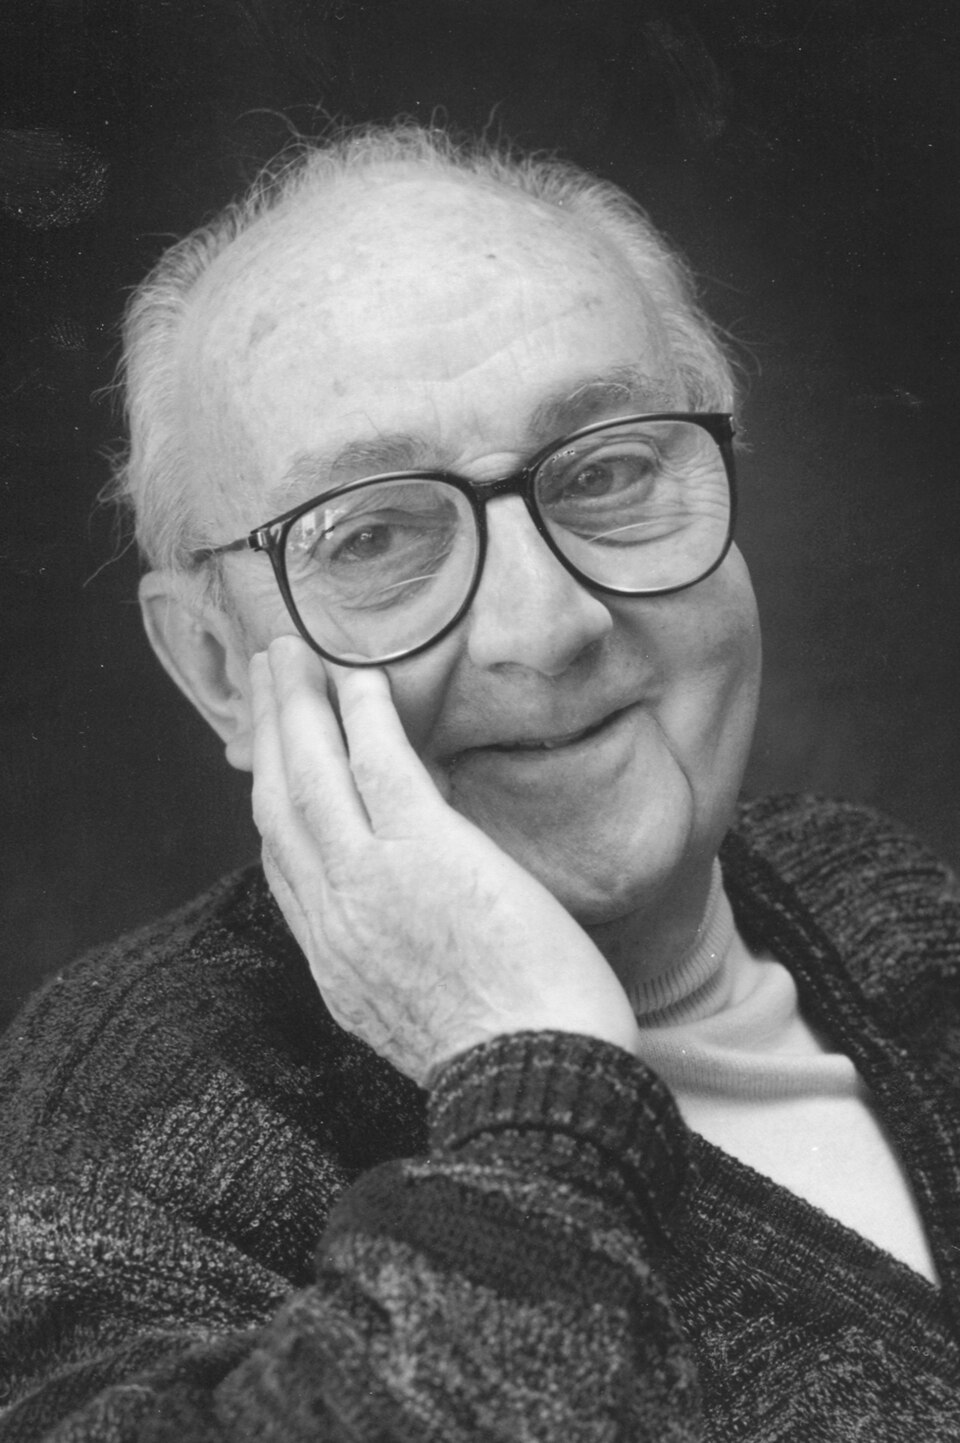
\includegraphics[height=0.42\textheight]{ch0_box.jpg}\\[1mm]
\imgcap{George E. P. Box (1919--2013)}
\imgcredit{https://commons.wikimedia.org/wiki/File:GeorgeEPBox_(cropped).jpg}{Photo: DavidMCEddy (2011); CC BY-SA 3.0; Wikimedia Commons}
\end{column}
\end{columns}
\end{frame}

\begin{frame}{Step 1: the data}
\itemsize{\footnotesize}
\begin{center}
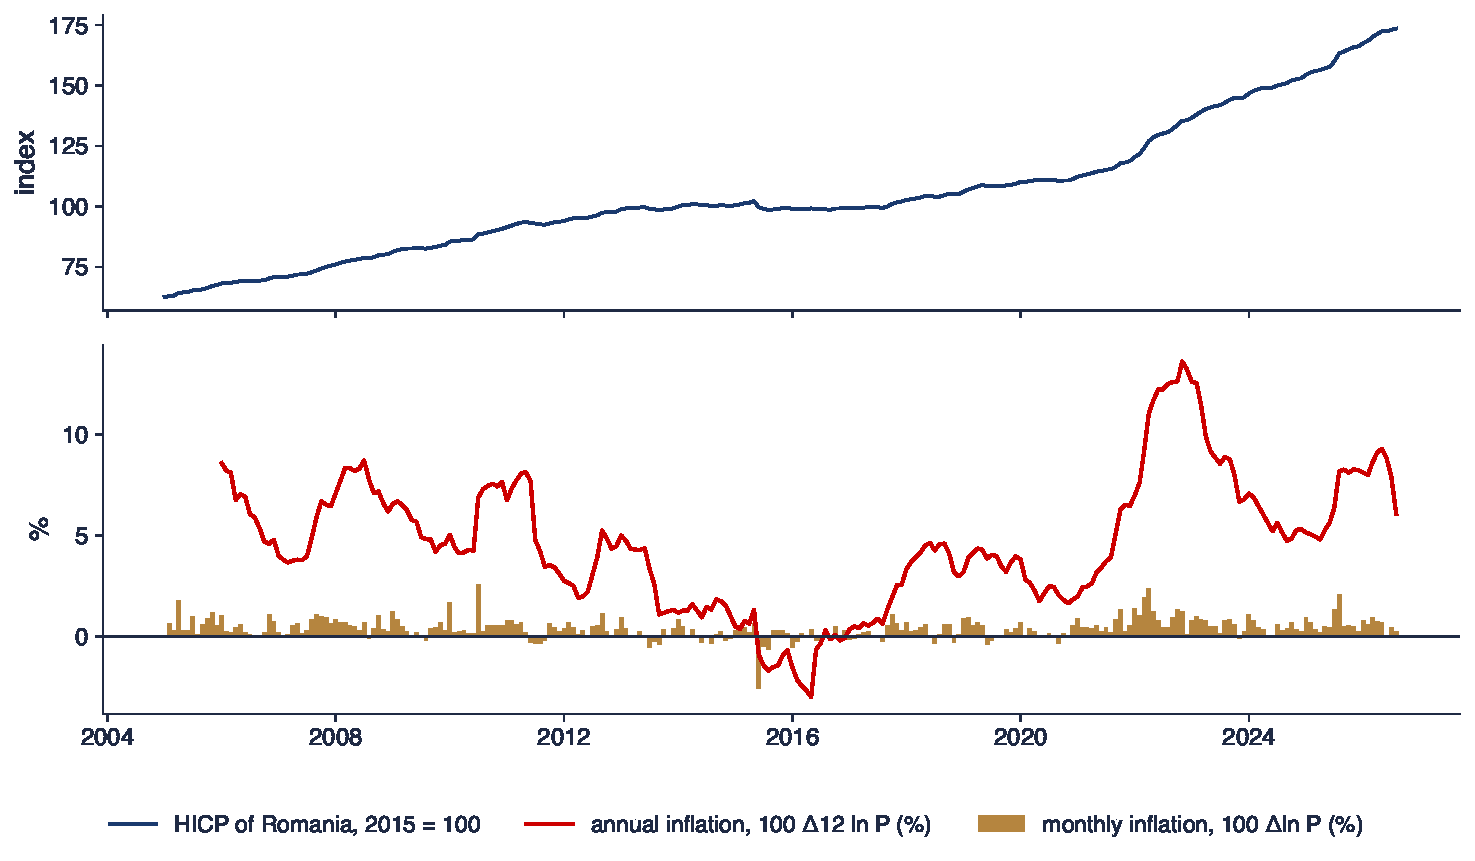
\includegraphics[width=0.97\textwidth,height=0.6\textheight,keepaspectratio]{tsa_ch15_bj_data.pdf}
\end{center}
\vspace{-0.25cm}
\begin{itemize}
    \item Top: HICP, 2015 = 100; bottom: monthly inflation $100\Delta\ln P_t$ (bars) and annual inflation $100\Delta_{12}\ln P_t$ (line)
\end{itemize}
\quantlet{TSA\_ch15\_box\_jenkins}{\qlurl{TSA_ch15_box_jenkins}}
\end{frame}

\begin{frame}{Interpreting the data}
\itemsize{\small}
\begin{itemize}
    \item \textbf{Trend}
    \begin{itemize}
        \item the index rises almost every month
        \item the logarithm is the natural scale
        \item monthly inflation averages 0.39\%; annual inflation ranges from $\ensuremath{-}3.0\%$ (May 2016) to 13.6\% (November 2022)
    \end{itemize}
    \item \textbf{Seasonality}
    \begin{itemize}
        \item January averages 0.74\%, June $\ensuremath{-}0.03\%$ (fresh food)
        \item a seasonal pattern in $\Delta\ln P_t$: we will need $\Delta_{12}$ or seasonal terms
    \end{itemize}
    \item \textbf{Shocks}
    \begin{itemize}
        \item tax changes move prices in one month
        \item July--August 2025: end of the electricity price caps and a higher VAT; annual inflation from 6.4\% to 8.2\%
    \end{itemize}
\end{itemize}
\end{frame}

\begin{frame}{Step 2: unit-root and stationarity tests}
\itemsize{\footnotesize}
\begin{center}
\footnotesize
\begin{tabular}{lccccc}
\toprule
\textbf{Series} & \textbf{Terms} & ADF $\tau$ & $p$ & KPSS $\eta$ (5\%: crit.) & \textbf{Verdict} \\
\midrule
$100\ln P_t$ & const., trend & $\ensuremath{-}0.96$ & 0.949 & 0.314 (0.146) & unit root \\
$\Delta\ln P_t$ & const. & $\ensuremath{-}4.00$ & 0.001 & 0.431 (0.463) & stationary, seasonal \\
$\Delta_{12}\ln P_t$ & const. & $\ensuremath{-}1.69$ & 0.435 & 0.424 (0.463) & inconclusive \\
$z_t = \Delta\Delta_{12}\ln P_t$ & const. & $\ensuremath{-}4.83$ & $<$\,0.001 & 0.113 (0.463) & stationary \\
\bottomrule
\end{tabular}
\end{center}
\begin{itemize}
    \item ADF: $H_0$ unit root, lags by AIC \refDF; KPSS: $H_0$ stationarity \refKPSS; 5\% ADF critical values $\ensuremath{-}3.43$ (with trend), $\ensuremath{-}2.87$ (constant)
    \item Annual inflation: neither ADF nor KPSS rejects: an inconclusive result, as in \tsachlink{https://danpele.github.io/Time-Series-Analysis/EN/Courses/chapter3_unit_roots_arima_models.pdf}{Chapter 3}
    \item Decision: $d = 1$, $D = 1$: we model $z_t$, both tests agree that it is stationary
\end{itemize}\quantlet{TSA\_ch15\_box\_jenkins}{\qlurl{TSA_ch15_box_jenkins}}
\end{frame}

\begin{frame}{Step 3: identification from the correlogram of $z_t$}
\itemsize{\footnotesize}
\begin{center}
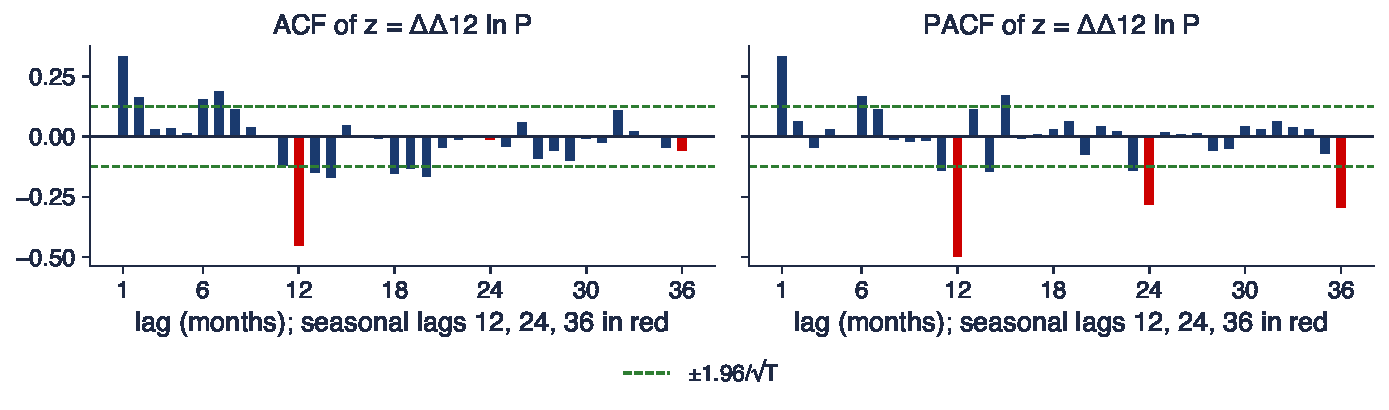
\includegraphics[width=0.97\textwidth,height=0.55\textheight,keepaspectratio]{tsa_ch15_bj_acf.pdf}
\end{center}
\vspace{-0.25cm}
\begin{itemize}
    \item ACF and PACF of $z_t = \Delta\Delta_{12}\ln P_t$, lags 1--36, $T = 247$; seasonal lags in red; band $\pm 0.125$
\end{itemize}
\quantlet{TSA\_ch15\_box\_jenkins}{\qlurl{TSA_ch15_box_jenkins}}
\end{frame}

\begin{frame}{Interpreting the correlogram}
\itemsize{\small}
\begin{itemize}
    \item \textbf{Regular part}
    \begin{itemize}
        \item $\hat\rho_1 = 0.33$, $\hat\rho_2 = 0.16$
        \item PACF $\hat\phi_{11} = 0.33$, then small: an AR(1)
        \item an MA(1) is also possible: ACF and PACF both shrink after lag 1
    \end{itemize}
    \item \textbf{Seasonal part}
    \begin{itemize}
        \item ACF $\ensuremath{-}0.45$ at lag 12, then $\ensuremath{-}0.01$ at 24
        \item PACF $\ensuremath{-}0.50$, $\ensuremath{-}0.28$, $\ensuremath{-}0.29$ at 12, 24, 36
        \item one seasonal ACF spike and a decaying seasonal PACF: a seasonal MA(1)
    \end{itemize}
    \item First candidate: SARIMA$(1,1,0)(0,1,1)_{12}$ for $\ln P_t$; the satellites at lags 11 and 13 are the product $\rho_1\rho_{12}$
\end{itemize}
\end{frame}

\begin{frame}{Step 4: estimating the candidates}
\itemsize{\footnotesize}
\begin{center}
\footnotesize
\begin{tabular}{lccccc}
\toprule
\textbf{Model} & param. & AICc & BIC & LB(12) $p$ & LB(24) $p$ \\
\midrule
$(1,1,0)(0,1,1)_{12}$, identified & 3 & 295.2 & 305.3 & 0.004 & 0.004 \\
${(1,1,1)(0,1,1)}_{12}$ & 4 & 285.4 & 298.9 & 0.029 & 0.088 \\
${(2,1,1)(0,1,1)}_{12}$ & 5 & 282.6 & 299.4 & 0.233 & 0.237 \\
${(1,1,2)(0,1,1)}_{12}$ & 5 & 282.8 & 299.6 & 0.233 & 0.217 \\
${(1,1,1)(1,1,1)}_{12}$ & 5 & 287.7 & 304.5 & 0.017 & 0.070 \\
\bottomrule
\end{tabular}
\end{center}
\begin{itemize}
    \item All 36 SARIMA$(p,1,q)(P,1,Q)_{12}$ with $p, q \le 2$, $P, Q \le 1$, on the training sample to August 2024 ($T = 236$); sorted by BIC
    \item param.: all estimated parameters, the variance included; Ljung--Box on the residuals with $m - k$ degrees of freedom, $k$ = the ARMA parameters
    \item The identified model fails the residual check; the lowest BIC, $(1,1,1)(0,1,1)$, fails at lag 12; the chosen model is $(2,1,1)(0,1,1)_{12}$, the lowest BIC among the models that pass
\end{itemize}\quantlet{TSA\_ch15\_box\_jenkins}{\qlurl{TSA_ch15_box_jenkins}}
\end{frame}

\begin{frame}{Step 4: the chosen model}
\itemsize{\footnotesize}
\begin{center}
\footnotesize
\begin{tabular}{lcccc}
\toprule
\textbf{Parameter} & \textbf{Estimate} & SE & $z$ & $p$ \\
\midrule
$\phi_1$ (ar.L1) & $1.156$ & $0.149$ & $7.76$ & $<$\,0.001 \\
$\phi_2$ (ar.L2) & $\ensuremath{-}0.183$ & $0.122$ & $\ensuremath{-}1.50$ & 0.133 \\
$\theta_1$ (ma.L1) & $\ensuremath{-}0.856$ & $0.099$ & $\ensuremath{-}8.61$ & $<$\,0.001 \\
$\Theta_1$ (ma.S.L12) & $\ensuremath{-}0.935$ & $0.098$ & $\ensuremath{-}9.55$ & $<$\,0.001 \\
$\sigma^2$ & $0.179$ & & & \\
\bottomrule
\end{tabular}
\end{center}
\begin{itemize}
    \item $(1 - \phi_1L - \phi_2L^2)\,z_t = (1 + \theta_1L)(1 + \Theta_1L^{12})\,\varepsilon_t$, $z_t = \Delta\Delta_{12}\,100\ln P_t$
    \item $\hat\Theta_1$ close to $-1$: the seasonal pattern is almost fixed, $\Delta_{12}$ nearly cancels; seasonal dummies would be an alternative
    \item The smallest AR root has modulus 1.034: inflation shocks are very persistent, as in \tsachlink{https://danpele.github.io/Time-Series-Analysis/EN/Courses/chapter2_arma_models.pdf}{Chapters 2} and \tsachlink{https://danpele.github.io/Time-Series-Analysis/EN/Courses/chapter8_long_memory_arfima.pdf}{8}
\end{itemize}\quantlet{TSA\_ch15\_box\_jenkins}{\qlurl{TSA_ch15_box_jenkins}}
\end{frame}

\begin{frame}{Step 5: checking the residuals}
\itemsize{\footnotesize}
\begin{center}
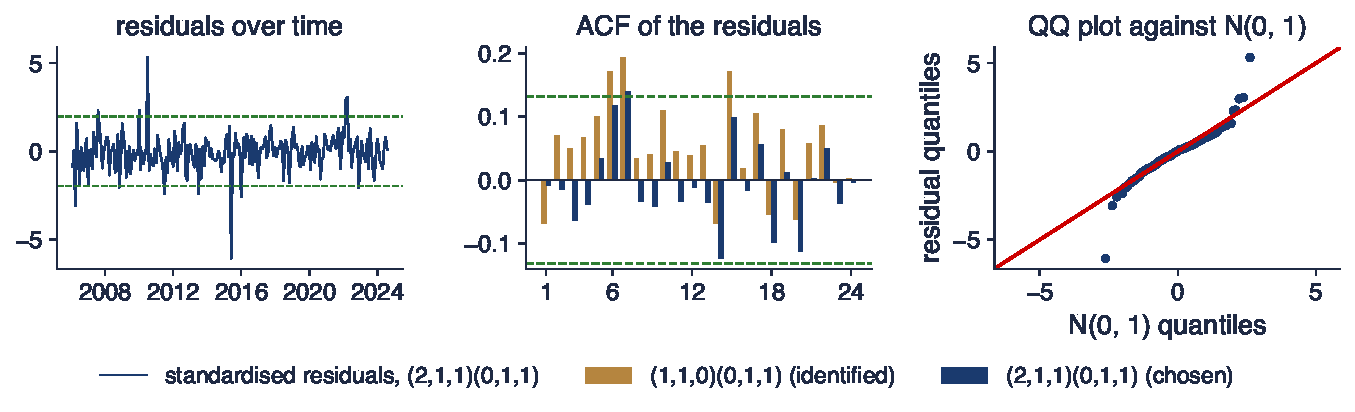
\includegraphics[width=0.97\textwidth,height=0.55\textheight,keepaspectratio]{tsa_ch15_bj_diag.pdf}
\end{center}
\vspace{-0.25cm}
\begin{itemize}
    \item Standardised residuals of the chosen model; ACF of the residuals of both models; QQ plot against $N(0, 1)$
\end{itemize}
\quantlet{TSA\_ch15\_box\_jenkins}{\qlurl{TSA_ch15_box_jenkins}}
\end{frame}

\begin{frame}{Interpreting the residual checks}
\itemsize{\small}
\begin{itemize}
    \item \textbf{No autocorrelation left}
    \begin{itemize}
        \item Ljung--Box $Q(12) = 10.49$ ($8$ df, $p = 0.233$), $Q(24) = 24.13$ ($p = 0.237$)
        \item the identified model had $p = 0.004$ and 0.004: the extra AR and MA terms reduce the autocorrelation at lags 6--7
    \end{itemize}
    \item \textbf{Not Normal}
    \begin{itemize}
        \item Jarque--Bera 450, kurtosis 9.9
        \item the two largest residuals: June 2015 ($\ensuremath{-}6.1\sigma$, the VAT cut on food) and July 2010 ($5.3\sigma$, the VAT increase)
    \end{itemize}
    \item Consequence: point forecasts are fine, Normal intervals are too narrow when taxes change; dummies for known tax changes would help
\end{itemize}
\end{frame}

\begin{frame}{Step 6: forecasts}
\itemsize{\footnotesize}
\begin{center}
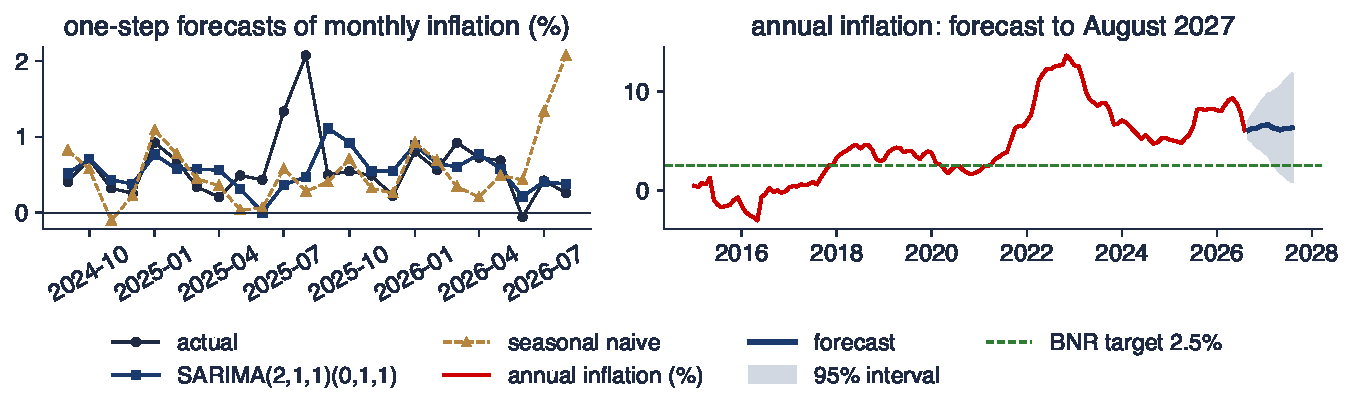
\includegraphics[width=0.97\textwidth,height=0.55\textheight,keepaspectratio]{tsa_ch15_bj_forecast.pdf}
\end{center}
\vspace{-0.25cm}
\begin{itemize}
    \item Left: one-step forecasts of monthly inflation on the test sample (September 2024 -- August 2026), parameters fixed at the training estimates; right: annual inflation forecasts to August 2027 with 95\% intervals, model re-estimated on all data
\end{itemize}
\quantlet{TSA\_ch15\_box\_jenkins}{\qlurl{TSA_ch15_box_jenkins}}
\end{frame}

\begin{frame}{Interpreting the forecasts}
\itemsize{\footnotesize}
\begin{center}
\footnotesize
\begin{tabular}{lccc}
\toprule
\textbf{Monthly inflation, test sample} & RMSE & MAE & MASE \\
\midrule
SARIMA$(2,1,1)(0,1,1)_{12}$ & 0.45 & 0.28 & 0.66 \\
seasonal naive & 0.64 & 0.42 & 0.99 \\
naive & 0.51 & 0.38 & 0.88 \\
\bottomrule
\end{tabular}
\end{center}
\begin{itemize}
    \item SARIMA has the smallest errors, but Diebold--Mariano (HLN) does not reject equal accuracy: $\ensuremath{-}1.40$ ($p = 0.174$) against the seasonal naive, $\ensuremath{-}0.47$ ($p = 0.642$) against the naive method
    \begin{itemize}
        \item 24 months are few; the largest misses: August 2025 (2.07\% against 0.47\%) and July 2025 (1.34\% against 0.37\%): tax and energy decisions that no univariate model can foresee
    \end{itemize}
    \item Annual inflation: 6.1\% in August 2026; forecast 6.1\% for September 2026 [5.3, 6.9], 6.3\% for August 2027 [0.9, 11.8]
    \begin{itemize}
        \item the August 2025 VAT jump leaves the 12-month window in August 2026; the 12-month interval is wide: a near unit root in $\Delta\ln P_t$
    \end{itemize}
\end{itemize}\quantlet{TSA\_ch15\_box\_jenkins}{\qlurl{TSA_ch15_box_jenkins}}
\end{frame}

\begin{frame}{Recap: Box--Jenkins on Romanian inflation}
\itemsize{\small}
\begin{itemize}
    \item Plot, transform, test: $\ln P_t$ needs $d = 1$ and $D = 1$
    \item The correlogram suggests $(1,1,0)(0,1,1)_{12}$; the residual check rejects it; the chosen model is $(2,1,1)(0,1,1)_{12}$
    \item Out of sample the gain over the seasonal naive method is not significant; tax shocks dominate the errors
\end{itemize}
\end{frame}


%=============================================================================
\section{The exam}
%=============================================================================

\begin{frame}{The written exam: format}
\itemsize{\small}
\begin{columns}[T]
\begin{column}{0.58\textwidth}
\begin{itemize}
    \item \textbf{70\% of the final grade}; written, 2 hours
    \begin{itemize}
        \item five subjects, all compulsory; 9 points for the subjects plus 1 point ex officio
    \end{itemize}
    \item \textbf{Three kinds of subjects}
    \begin{itemize}
        \item a short derivation: moments, stationarity, the ACF or the form of a process
        \item the interpretation of software output: estimates, tests, correlograms, VAR and VECM tables
        \item model choice and a forecast computed by hand from the output
    \end{itemize}
    \item The critical values you need are printed in the output, as in the problems below
\end{itemize}
\end{column}
\begin{column}{0.38\textwidth}
\centering
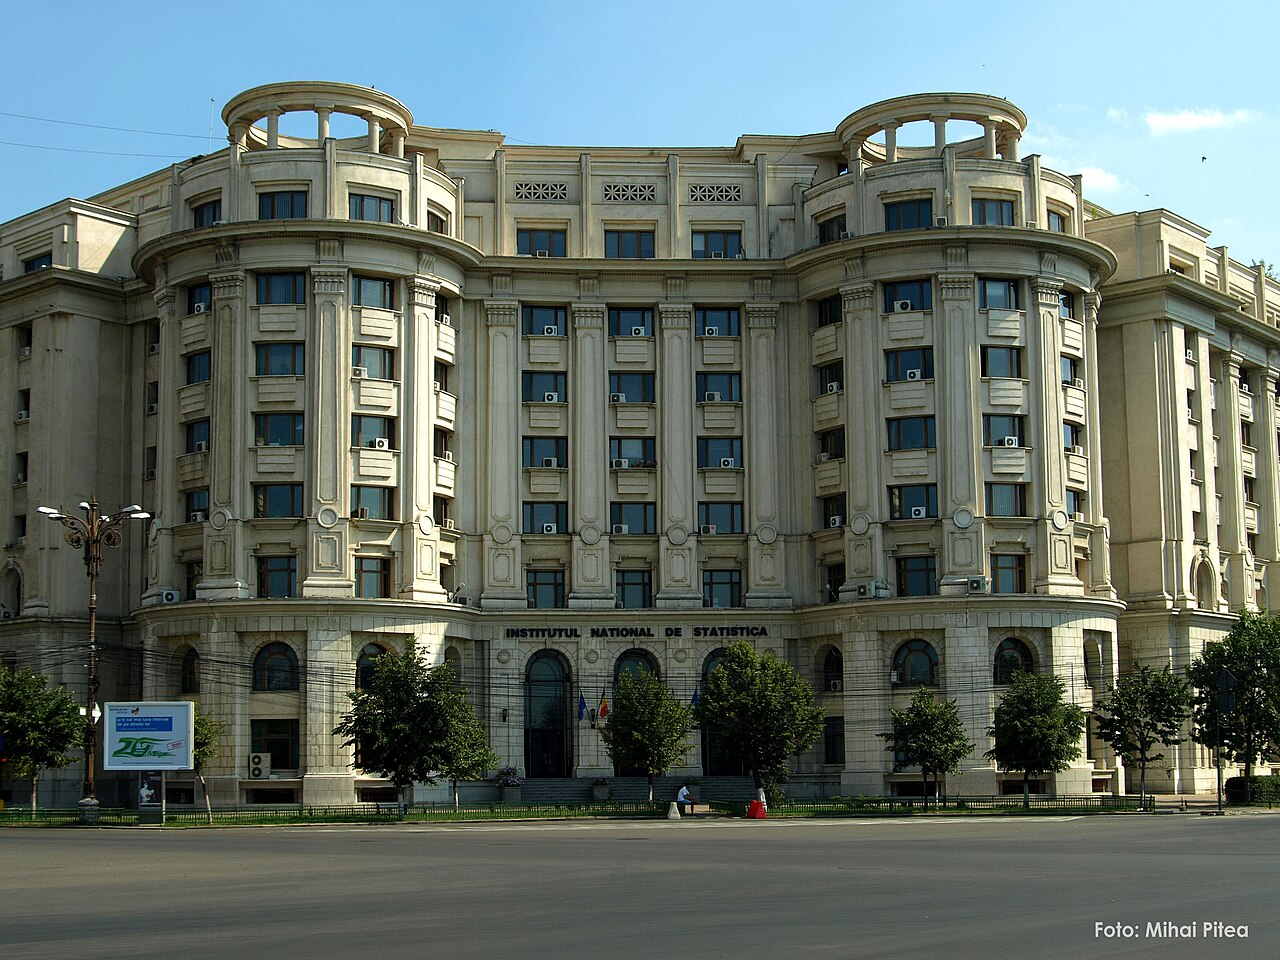
\includegraphics[height=0.40\textheight]{ch2_ins_bucharest_2009.jpg}\\[1mm]
\imgcap{The National Institute of Statistics, Bucharest: the source of many exam series}
\imgcredit{https://commons.wikimedia.org/wiki/File:Institutul_Na\%C8\%9Bional_de_Statistic\%C4\%83.jpg}{Photo: Dan Mihai Pitea (2009); CC BY-SA 3.0; Wikimedia Commons}
\end{column}
\end{columns}
\end{frame}

\begin{frame}{Content assessed}
\itemsize{\small}
\begin{itemize}
    \item \textbf{\tsachlink{https://danpele.github.io/Time-Series-Analysis/EN/Courses/chapter0_introduction.pdf}{Chapters 0}--\tsachlink{https://danpele.github.io/Time-Series-Analysis/EN/Courses/chapter10_state_space_kalman_markov_switching.pdf}{10}}
    \begin{itemize}
        \item lectures and seminars
        \item the definitions and formulas of the ``Prerequisites for Today'' slides of every seminar
        \item the computations of Part A of the seminars, on paper
    \end{itemize}
    \item \textbf{Reading output}
    \begin{itemize}
        \item tables like those of Part B and of this chapter
        \item EViews or Python output: the same numbers under different names (AR(1), ar.L1; SAR(12), ar.S.L12)
        \item no code is written at the exam
    \end{itemize}
    \item \textbf{Core weight}
    \begin{itemize}
        \item ARIMA and SARIMA, unit roots, VAR and Granger causality, cointegration and VECM, GARCH
        \item \tsachlink{https://danpele.github.io/Time-Series-Analysis/EN/Courses/chapter11_foundation_models_time_series.pdf}{Chapters 11}--\tsachlink{https://danpele.github.io/Time-Series-Analysis/EN/Courses/chapter14_multivariate_garch_models.pdf}{14} are for self-study (not examined unless the instructor decides otherwise)
    \end{itemize}
\end{itemize}
\end{frame}

\begin{frame}{Grading criteria}
\itemsize{\small}
\begin{itemize}
    \item \textbf{The method}
    \begin{itemize}
        \item the formula or the equation, with the numbers substituted
        \item a correct method with an arithmetic slip receives most of the points
    \end{itemize}
    \item \textbf{The result}
    \begin{itemize}
        \item the number with its unit (\%, percentage points, months) and its sign
        \item for a test: $H_0$, the statistic, the critical value or the $p$-value, the decision
    \end{itemize}
    \item \textbf{The interpretation}
    \begin{itemize}
        \item three to five sentences, statistical and economic
        \item a correct number with a wrong interpretation does not receive all the points
        \item say what the model cannot show (causality, structural breaks, the future of policy)
    \end{itemize}
\end{itemize}
\end{frame}

\begin{frame}{Typical problem types}
\itemsize{\small}
\begin{center}
\footnotesize
\begin{tabular}{>{\raggedright\arraybackslash}p{4.6cm}>{\raggedright\arraybackslash}p{1.4cm}>{\raggedright\arraybackslash}p{5.2cm}}
\toprule
\textbf{Type} & \textbf{Chapters} & \textbf{Example in this chapter} \\
\midrule
derivation: moments, stationarity, differencing & 1--3 & Problem 1: trend plus AR(1) errors \\
correlogram and unit-root output: identification & 1--3 & Problem 2: Romanian GDP \\
SARIMA output and a forecast by hand & 2--4 & Problem 3: Romanian inflation \\
VAR and Granger output & 6 & Problem 4: growth, inflation, ROBOR \\
cointegration and VECM output & 7 & Problem 5: US yields \\
GARCH output and VaR 1\% & 5 & Problem 6: the BET \\
forecast evaluation; state space and regimes & 4, 8--10 & Problems 7 and 8 \\
\bottomrule
\end{tabular}
\end{center}
\begin{itemize}
    \item The eight problems below are review examples with full solutions; the exam has its own subjects
\end{itemize}
\end{frame}

\begin{frame}{Problem 1: a trend with AR(1) errors}
\itemsize{\footnotesize}
\begin{itemize}
    \item \textbf{Context}
    \begin{itemize}
        \item $Y_t = 10 + 0.5t + u_t$, $u_t = 0.6u_{t-1} + \varepsilon_t$, $\varepsilon_t \sim WN(0, 1)$
        \item At $T = 100$ we observe $Y_T = 62$
    \end{itemize}
    \item \textbf{Tasks}
\begin{enumerate}
    \item Compute $E(Y_t)$ and $\mathrm{Var}(Y_t)$ and say whether $Y_t$ is stationary.
    \item Show that $\Delta Y_t$ is an ARMA(1,1) with $\theta = -1$ and compute $\rho_{\Delta Y}(1)$.
    \item Forecast $Y_{T+1}$ and $Y_{T+10}$ with the correct model and give the variance of the 10-step error.
    \item Explain what goes wrong if the analyst differences $Y_t$.
\end{enumerate}
\end{itemize}
\end{frame}

\begin{frame}{Problem 1: solution}
\itemsize{\footnotesize}
\begin{enumerate}
    \item $E(Y_t) = 10 + 0.5t$ depends on $t$: not stationary; $\mathrm{Var}(Y_t) = 1/(1 - 0.36) = 1.5625$ is constant: \textbf{trend-stationary}
    \item $\Delta Y_t = 0.5 + \Delta u_t$ and $(1 - 0.6L)\Delta u_t = (1 - L)\varepsilon_t$: ARMA(1,1), $\theta = -1$; $\gamma(0) = 1.25$, $\gamma(1) = \ensuremath{-}0.25$, $\rho(1) = \ensuremath{-}0.20$
    \item $u_T = 62 - 10 - 50 = 2.0$; $\hat Y_{T+1} = 10 + 50.5 + 0.6 \cdot 2 = 61.70$; $\hat Y_{T+10} = 10 + 55 + 0.6^{10} \cdot 2 = 65.01$; variance $(1 - 0.6^{20})/(1 - 0.36) = 1.562$
    \item The MA root is 1: $\Delta Y_t$ is not invertible, $\hat\rho_1 < 0$ and an MA coefficient near $-1$ are the signs of over-differencing
\end{enumerate}
\begin{itemize}
    \item \textbf{Interpretation}
    \begin{itemize}
        \item A shock dies out: after 10 periods only $0.012$ of the deviation is left, and the error variance stays bounded
        \item The treatment follows the type of trend: detrend a trend-stationary series, difference a series with a unit root (\tsachlink{https://danpele.github.io/Time-Series-Analysis/EN/Courses/chapter3_unit_roots_arima_models.pdf}{Chapter 3})
    \end{itemize}
\end{itemize}
\end{frame}

\begin{frame}{Problem 2: identifying Romanian GDP}
\itemsize{\footnotesize}
\begin{center}
\scriptsize
\begin{tabular}{lcccccc}
\toprule
\textbf{Series} & Terms & ADF $\tau$ & $p$ & crit. 1\%; 5\%; 10\% & KPSS & crit. 5\% \\
\midrule
$100\ln Y_t$ & c, t & $\ensuremath{-}2.31$ & 0.428 & $\ensuremath{-}4.05$; $\ensuremath{-}3.45$; $\ensuremath{-}3.15$ & 0.198 & 0.146 \\
$100\Delta\ln Y_t$ & c & $\ensuremath{-}10.77$ & $<$\,0.001 & $\ensuremath{-}3.49$; $\ensuremath{-}2.89$; $\ensuremath{-}2.58$ & 0.263 & 0.463 \\
\bottomrule
\end{tabular}
\end{center}
\begin{itemize}
    \item \textbf{Context}
    \begin{itemize}
        \item Romanian real GDP, seasonally adjusted (Eurostat), 2000Q1 -- 2026Q2
        \item Growth $g_t = 100\Delta\ln Y_t$: ACF $\ensuremath{-}0.05$, $\ensuremath{-}0.14$; PACF $\ensuremath{-}0.05$, $\ensuremath{-}0.14$ (lags 1, 2; band $\pm 0.19$); Ljung--Box $Q(8) = 7.28$, $p = 0.506$; $\chi^2_{0.95}(8) = 15.51$
    \end{itemize}
    \item \textbf{Tasks}
\begin{enumerate}
    \item Describe the ADF test and decide whether $\ln Y_t$ and $g_t$ are stationary.
    \item Say whether KPSS agrees.
    \item Identify the process with the Box--Jenkins method.
    \item The estimated drift is $0.81$ (SE $0.30$): write the model and interpret the drift.
\end{enumerate}
\end{itemize}
\end{frame}

\begin{frame}{Problem 2: solution}
\itemsize{\footnotesize}
\begin{enumerate}
    \item ADF: $\Delta y_t = c + bt + \gamma y_{t-1} + \sum\delta_j\Delta y_{t-j} + \varepsilon_t$, $H_0$: $\gamma = 0$ (unit root); $\ln Y_t$: $\ensuremath{-}2.31 > \ensuremath{-}3.45$: not rejected; $g_t$: $\ensuremath{-}10.77 < \ensuremath{-}3.49$: rejected
    \item KPSS ($H_0$: stationarity): $0.198 > 0.146$ rejects for the level, $0.263 < 0.463$ does not for growth: $\ln Y_t \sim I(1)$
    \item ACF and PACF of $g_t$ inside the band, $Q(8) = 7.28 < 15.51$: growth is white noise around its mean
    \item ARIMA(0,1,0) with drift: $100\ln Y_t = 100\ln Y_{t-1} + 0.81 + \varepsilon_t$, $\hat\sigma = 2.47$; $t = 2.72$
\end{enumerate}
\begin{itemize}
    \item \textbf{Interpretation}
    \begin{itemize}
        \item The economy grows by about 0.81\% a quarter, about 3.2\% a year; quarterly surprises are not predictable
        \item A shock to the level is permanent: the 2009 and 2020 recessions moved the path of GDP for good
    \end{itemize}
\end{itemize}
\end{frame}

\begin{frame}{Problem 3: SARIMA output and a forecast by hand}
\itemsize{\footnotesize}
\begin{center}
\scriptsize
\begin{tabular}{lcccc}
\toprule
\textbf{Dependent: $z_t$} & Coefficient & SE & $z$ & $p$ \\
\midrule
AR(1) & $0.353$ & $0.054$ & $6.53$ & $<$\,0.001 \\
SAR(12) & $\ensuremath{-}0.488$ & $0.035$ & $\ensuremath{-}13.90$ & $<$\,0.001 \\
SIGMASQ & $0.254$ & & & \\
Ljung--Box $Q(12)$ & $22.64$ & & & 0.012 \\
\bottomrule
\end{tabular}
\end{center}
\begin{itemize}
    \item \textbf{Context}
    \begin{itemize}
        \item $z_t = \Delta\Delta_{12}\,100\ln \mathrm{HICP}_t$ (``DLOG(IPC,1,12)''), Romania, February 2006 -- August 2026, $T = 247$
        \item Last values: $z$ = $\ensuremath{-}1.814$ (August 2026), $0.090$ (September 2025), $1.794$ (August 2025); annual inflation in August 2026: 6.085\%
    \end{itemize}
    \item \textbf{Tasks}
\begin{enumerate}
    \item Write the equation of the model and interpret the coefficients.
    \item Test whether the residuals are white noise.
    \item Forecast $z$ and the annual inflation rate for September 2026.
\end{enumerate}
\end{itemize}
\end{frame}

\begin{frame}{Problem 3: solution}
\itemsize{\scriptsize}
\begin{enumerate}
    \item $(1 - \phi L)(1 - \Phi L^{12})z_t = \varepsilon_t$, so $z_t = \phi z_{t-1} + \Phi z_{t-12} - \phi\Phi z_{t-13} + \varepsilon_t$
    \item $\hat\phi = 0.353$: a monthly surprise continues one month later; $\hat\Phi = \ensuremath{-}0.488 < 0$: a surprise in a month is partly reversed in the same month a year later; both significant; inverted AR roots 0.35 and 0.94 $< 1$: stationary
    \item Ljung--Box $Q(12) = 22.64$ on $12 - 2 = 10$ df, $p = 0.012$: white noise is rejected at 5\%; the model leaves some autocorrelation (compare Step 5 above)
    \item $\hat z_{T+1} = 0.353(\ensuremath{-}1.814) + (\ensuremath{-}0.488)(0.090) - (\ensuremath{-}0.173)(1.794) = \ensuremath{-}0.641 + (\ensuremath{-}0.044) + 0.310 = \ensuremath{-}0.375$
    \item Annual inflation: $\Delta_{12}\ln P_{T+1} = \Delta_{12}\ln P_T + z_{T+1} = 6.085 + (\ensuremath{-}0.375) = 5.71\%$
\end{enumerate}
\begin{itemize}
    \item \textbf{Interpretation}
    \begin{itemize}
        \item Inflation is expected to keep falling in September 2026 as last year's tax shock leaves the 12-month window
        \item Residual autocorrelation: a richer model (as in Step 4) would change the forecast slightly; a 95\% interval needs $\hat\sigma$
    \end{itemize}
\end{itemize}
\end{frame}

\begin{frame}{Problem 4: VAR output and Granger causality}
\itemsize{\scriptsize}
\begin{center}
\scriptsize
\begin{tabular}{lccc}
\toprule
\textbf{ROBOR equation} & coef. [$t$] & & coef. [$t$] \\
\midrule
$g_{t-1}$ & $0.142$ [$3.49$] & $g_{t-2}$ & $0.074$ [$1.73$] \\
$\pi_{t-1}$ & $0.240$ [$2.78$] & $\pi_{t-2}$ & $\ensuremath{-}0.172$ [$\ensuremath{-}1.89$] \\
$i_{t-1}$ & $1.042$ [$10.16$] & $i_{t-2}$ & $\ensuremath{-}0.119$ [$\ensuremath{-}1.20$] \\
constant & $\ensuremath{-}0.109$ [$\ensuremath{-}0.55$] & $R^2$ & 0.93 \\
\bottomrule
\end{tabular}
\end{center}
\begin{center}
\scriptsize
\begin{tabular}{lcc}
\toprule
\textbf{Null hypothesis} & $F$ & $p$ \\
\midrule
$g$ does not Granger-cause $i$ & 7.26 & 0.001 \\
$\pi$ does not Granger-cause $i$ & 4.74 & 0.011 \\
$i$ does not Granger-cause $\pi$ & 0.89 & 0.417 \\
\bottomrule
\end{tabular}
\end{center}
\begin{itemize}
    \item \textbf{Context}
    \begin{itemize}
        \item VAR(2) for Romania, 2005Q3 -- 2026Q2 ($T = 84$): GDP growth $g$, annual inflation $\pi$, ROBOR 3M $i$
    \end{itemize}
    \item \textbf{Tasks}
\begin{enumerate}
    \item Describe Granger causality and interpret the table.
    \item Write the ROBOR equation and quantify the long-run effect of a permanent 1 pp rise in inflation on ROBOR.
    \item Recompute the first $F$ from $RSS_R = 69.27$ and $RSS_U = 58.27$.
\end{enumerate}
\end{itemize}
\end{frame}

\begin{frame}{Problem 4: solution}
\itemsize{\scriptsize}
\begin{enumerate}
    \item $x$ Granger-causes $y$ if the lags of $x$ improve the forecast of $y$ given the lags of $y$ (joint $F$ test) \refGranger; growth and inflation help to forecast ROBOR ($p =$ 0.001 and 0.011); ROBOR does not help to forecast inflation ($p = 0.417$)
    \item $i_t = \ensuremath{-}0.109 + 0.142g_{t-1} + 0.074g_{t-2} + 0.240\pi_{t-1} + (\ensuremath{-}0.172)\pi_{t-2} + 1.042i_{t-1} + (\ensuremath{-}0.119)i_{t-2} + u_t$
    \item Long run ($i_t = i_{t-1}$, $\pi_t = \pi_{t-1}$): $\partial i/\partial\pi = (0.240 + (\ensuremath{-}0.172))/(1 - 1.042 - (\ensuremath{-}0.119)) = 0.068/0.076 = 0.90$ pp
    \item $F = \frac{(69.27 - 58.27)/2}{58.27/77} = 7.26 > F_{0.95}(2, 77) = 3.12$: $H_0$ rejected
\end{enumerate}
\begin{itemize}
    \item \textbf{Interpretation}
    \begin{itemize}
        \item The money market rate follows the economy and inflation, as a central bank reaction would imply; the reverse link is not visible in quarterly data
        \item The long-run effect divides by $0.076$, a number close to zero: it is imprecise; Granger causality is predictability, not proof of a policy effect
    \end{itemize}
\end{itemize}
\end{frame}

\begin{frame}{Problem 5: cointegration and VECM output}
\itemsize{\scriptsize}
\begin{center}
\scriptsize
\begin{tabular}{lcccc}
\toprule
\textbf{Johansen trace test} & $r = 0$ & $r \le 1$ & $r \le 2$ & \\
\midrule
statistic & 54.60 & 21.57 & 3.12 & \\
5\% critical value & 29.80 & 15.49 & 3.84 & \\
\bottomrule
\end{tabular}
\end{center}
\begin{center}
\scriptsize
\begin{tabular}{lccc}
\toprule
\textbf{Adjustment} $\alpha$ [$t$] & $\Delta y^{(1)}$ & $\Delta y^{(5)}$ & $\Delta y^{(10)}$ \\
\midrule
EC1 & $\ensuremath{-}0.021$ [$\ensuremath{-}0.82$] & $0.045$ [$2.21$] & $0.040$ [$2.22$] \\
EC2 & $0.024$ [$0.31$] & $\ensuremath{-}0.122$ [$\ensuremath{-}2.00$] & $\ensuremath{-}0.077$ [$\ensuremath{-}1.43$] \\
\bottomrule
\end{tabular}
\end{center}
\begin{itemize}
    \item \textbf{Context}
    \begin{itemize}
        \item US Treasury yields at 1, 5 and 10 years (monthly, FRED), January 1960 -- September 2026, VECM with two lagged differences
        \item Cointegrating equations: EC1 $= y^{(1)}_{t-1} - 1.045\,y^{(10)}_{t-1} + 1.223$; EC2 $= y^{(5)}_{t-1} - 1.044\,y^{(10)}_{t-1} + 0.587$
    \end{itemize}
    \item \textbf{Tasks}
\begin{enumerate}
    \item Define cointegration and decide the rank.
    \item Write the error-correction part of the equation for $\Delta y^{(10)}_t$ and say which yields adjust.
    \item Interpret the long-run relations economically.
\end{enumerate}
\end{itemize}
\end{frame}

\begin{frame}{Problem 5: solution}
\itemsize{\scriptsize}
\begin{enumerate}
    \item $I(1)$ series are cointegrated if a linear combination is $I(0)$ \refEG; trace: $54.60 > 29.80$, $21.57 > 15.49$, $3.12 < 3.84$: rank $r = 2$, one common stochastic trend \refJoh
    \item $\Delta y^{(10)}_t = 0.040\,\mathrm{EC1}_{t-1} + (\ensuremath{-}0.077)\,\mathrm{EC2}_{t-1} + \dots$; on EC1 the 5- and 10-year yields have $|t| > 2$, the 1-year yield $|t| < 1$ on both relations: the short rate does not adjust (weakly exogenous)
    \item $\beta \approx 1$: the spreads $y^{(1)} - y^{(10)}$ and $y^{(5)} - y^{(10)}$ are stationary, as the expectations hypothesis implies; half-lives of the equilibrium errors 22.1 and 9.0 months
\end{enumerate}
\begin{itemize}
    \item \textbf{Interpretation}
    \begin{itemize}
        \item The three yields share one trend (the level of rates); the curve can bend, but spreads return to their means
        \item The long rates do the adjusting: markets move the long end toward the policy-driven short end
    \end{itemize}
\end{itemize}
\end{frame}

\begin{frame}{Problem 6: GARCH output and VaR 1\%}
\itemsize{\footnotesize}
\begin{center}
\scriptsize
\begin{tabular}{lccccc}
\toprule
\textbf{BET} & $\mu$ & $\omega$ & $\alpha$ & $\beta$ & $\nu$ \\
\midrule
estimate & $0.083$ & $0.0448$ & $0.192$ & $0.799$ & $5.011$ \\
SE & $0.010$ & $0.0088$ & $0.025$ & $0.024$ & $0.308$ \\
\bottomrule
\end{tabular}
\end{center}
\begin{itemize}
    \item \textbf{Context}
    \begin{itemize}
        \item GARCH(1,1) with Student-$t$ innovations for daily BET log returns in \%, since 2000 ($n = 6\,670$)
        \item Today: $\sigma_t^2 = 1.0$ and $\varepsilon_t = -3.0$; $t_5^{-1}(0.01) = \ensuremath{-}3.365$; about 250 trading days a year
    \end{itemize}
    \item \textbf{Tasks}
\begin{enumerate}
    \item Compute the persistence, the half-life and the long-run annual volatility.
    \item Compute $\sigma_{t+1}^2$.
    \item Compute the one-day VaR 1\% with the standardised $t_5$ quantile and compare it with the Normal one.
\end{enumerate}
\end{itemize}
\end{frame}

\begin{frame}{Problem 6: solution}
\itemsize{\footnotesize}
\begin{enumerate}
    \item $\alpha + \beta = 0.991$; $h_{1/2} = \ln 0.5/\ln 0.991 = 74$ days; $\bar\sigma^2 = 0.0448/(1 - 0.991) = 4.82$, $\sqrt{250 \times 4.82} = 34.7\%$ a year
    \item $\sigma_{t+1}^2 = 0.0448 + 0.192 \times 9 + 0.799 \times 1.0 = 0.0448 + 1.725 + 0.799 = 2.568$, $\sigma_{t+1} = 1.603\%$
    \item $q_{0.01}(z) = \ensuremath{-}3.365 \times \sqrt{3/5} = \ensuremath{-}3.365 \times 0.775 = \ensuremath{-}2.606$; VaR 1\% $= -(0.083 + 1.603 \times (\ensuremath{-}2.606)) = 4.09\%$; Normal: $3.65\%$
\end{enumerate}
\begin{itemize}
    \item \textbf{Interpretation}
    \begin{itemize}
        \item Persistence close to 1: a shock to volatility halves only after about 74 trading days
        \item The long-run volatility (34.7\%) is far above the sample one (22.1\%): when $\alpha + \beta \approx 1$, $\omega/(1 - \alpha - \beta)$ is very imprecise
        \item Heavy tails raise VaR 1\% above the Normal value: a loss larger than 4.09\% is expected on one day in 100
    \end{itemize}
\end{itemize}
\end{frame}

\begin{frame}{Problem 7: evaluating forecasts}
\itemsize{\footnotesize}
\begin{center}
\scriptsize
\begin{tabular}{lcccccc}
\toprule
\textbf{Test month} & 1 & 2 & 3 & 4 & 5 & 6 \\
\midrule
errors, SARIMA & $0.3$ & $-0.5$ & $0.2$ & $0.6$ & $-0.4$ & $0.1$ \\
errors, seasonal naive & $0.5$ & $-0.7$ & $0.6$ & $0.4$ & $-0.9$ & $0.3$ \\
\bottomrule
\end{tabular}
\end{center}
\begin{itemize}
    \item \textbf{Context}
    \begin{itemize}
        \item Monthly inflation forecasts on a test sample of six months; the in-sample MAE of the seasonal naive method is 0.6
        \item A colleague reports $R^2 = 0.37$ for a boosting model of daily S\&P 500 returns, with random 5-fold cross-validation
    \end{itemize}
    \item \textbf{Tasks}
\begin{enumerate}
    \item Compute RMSE, MAE and MASE for both methods.
    \item Compute the Diebold--Mariano statistic on squared errors, $\bar d/(s_d/\sqrt{n})$, and decide at 5\% ($t_{0.975}(5) = 2.571$).
    \item Comment on the colleague's $R^2$.
\end{enumerate}
\end{itemize}
\end{frame}

\begin{frame}{Problem 7: solution}
\itemsize{\footnotesize}
\begin{enumerate}
    \item SARIMA: RMSE 0.389, MAE 0.350, MASE 0.58; seasonal naive: RMSE 0.600, MAE 0.567, MASE 0.94
    \item $d_t = e_{A,t}^2 - e_{B,t}^2$: $\ensuremath{-}0.16$, $\ensuremath{-}0.24$, $\ensuremath{-}0.32$, $0.20$, $\ensuremath{-}0.65$, $\ensuremath{-}0.08$; $\bar d = \ensuremath{-}0.208$, $s_d = 0.281$; DM $= \ensuremath{-}1.82$, $|\ensuremath{-}1.82| < 2.571$: equal accuracy is not rejected
    \item Random folds put future days in the training set: leakage; walk-forward validation gives $R^2 = \ensuremath{-}0.39$ for the same model (\tsachlink{https://danpele.github.io/Time-Series-Analysis/EN/Courses/chapter9_machine_learning_time_series.pdf}{Chapter 9})
\end{enumerate}
\begin{itemize}
    \item \textbf{Interpretation}
    \begin{itemize}
        \item MASE below 1: SARIMA beats the seasonal naive method on average, but six months cannot show that the gain is real
        \item Only out-of-sample, time-ordered evaluation counts as evidence of forecasting skill
    \end{itemize}
\end{itemize}
\end{frame}

\begin{frame}{Problem 8: state space, regimes and long memory}
\itemsize{\footnotesize}
\begin{itemize}
    \item \textbf{Context}
    \begin{itemize}
        \item Local level model: $\sigma^2_\varepsilon = 4$, $\sigma^2_\eta = 1$; prediction $a_t = 10$, $P_t = 2$; observation $y_t = 13$
        \item Romanian GDP growth, two regimes: $p_{11} = 0.911$ (volatile), $p_{22} = 0.934$ (stable) (\tsachlink{https://danpele.github.io/Time-Series-Analysis/EN/Courses/chapter10_state_space_kalman_markov_switching.pdf}{Chapter 10})
        \item Romanian monthly inflation: ARFIMA(0,$d$,0) with $\hat d = 0.31$ (SE 0.05) (\tsachlink{https://danpele.github.io/Time-Series-Analysis/EN/Courses/chapter8_long_memory_arfima.pdf}{Chapter 8})
    \end{itemize}
    \item \textbf{Tasks}
\begin{enumerate}
    \item Run one Kalman update and prediction; compute the steady-state gain and the equivalent SES weight.
    \item Compute the expected durations of the two regimes and the long-run share of the volatile regime.
    \item Compute $H$ and $\rho(1)$ for the ARFIMA model and say whether inflation is stationary and mean-reverting.
\end{enumerate}
\end{itemize}
\end{frame}

\begin{frame}{Problem 8: solution}
\itemsize{\footnotesize}
\begin{enumerate}
    \item $F_t = 2 + 4 = 6$, $K_t = 2/6 = 0.333$; $a_{t|t} = 10 + 0.333 \times 3 = 11.00$, $P_{t|t} = 2(1 - 0.333) = 1.333$; $a_{t+1} = 11.00$, $P_{t+1} = 2.333$
    \item $q = 0.25$: $\bar P/\sigma^2_\varepsilon = (q + \sqrt{q^2 + 4q})/2 = 0.6404$, $\bar K = 0.6404/(1 + 0.6404) = 0.390 = \alpha_{SES}$
    \item $E(D_1) = 1/(1 - 0.911) = 11.2$ quarters, $E(D_2) = 15.2$ quarters; $\pi_1 = (1 - 0.934)/(2 - 0.911 - 0.934) = 0.425$
    \item $H = d + 0.5 = 0.81$; $\rho(1) = d/(1 - d) = 0.45$; $0 < d < 0.5$: stationary with long memory, mean-reverting
\end{enumerate}
\begin{itemize}
    \item \textbf{Interpretation}
    \begin{itemize}
        \item The filter moves the level one third of the way to the surprise; in the long run the weight is that of exponential smoothing
        \item In the long run Romanian growth is in the volatile regime about 42\% of the time: transition, 2009 and 2020
        \item Inflation shocks fade slowly, hyperbolically: forecasts return to the mean more slowly than those of an AR model
    \end{itemize}
\end{itemize}
\end{frame}

\begin{frame}{Recap: The exam}
\itemsize{\small}
\begin{itemize}
    \item Written, 2 hours, five subjects, 70\% of the grade; \tsachlink{https://danpele.github.io/Time-Series-Analysis/EN/Courses/chapter0_introduction.pdf}{Chapters 0}--\tsachlink{https://danpele.github.io/Time-Series-Analysis/EN/Courses/chapter10_state_space_kalman_markov_switching.pdf}{10}
    \item Points for the method, the result with its unit and sign, and the interpretation
    \item Practise with Part A of every seminar, with Seminar 15 and with the \href{https://danpele.github.io/Time-Series-Analysis/exam/practice/exam_problems_en.pdf}{practice set} (25 problems with numerical answers)
\end{itemize}
\end{frame}


%=============================================================================
\section{The team project and attendance}
%=============================================================================

\begin{frame}{The team project: content and deliverables}
\itemsize{\small}
\begin{itemize}
    \item \textbf{20\% of the final grade}
    \begin{itemize}
        \item a team of 2--4 students analyses real series with the methods of the course
        \item one concrete question: forecasting EUR/RON, modelling Romanian inflation, monetary policy and bank rates
        \item one series: trend and stationarity, smoothing, ARIMA or SARIMA, a training set, a test set and a horizon, point and interval forecasts, two methods compared
        \item several series: unit roots, cointegration, VAR or VECM, Granger causality, IRF and FEVD
    \end{itemize}
    \item \textbf{Deliverables}
    \begin{itemize}
        \item a repository whose code reproduces every number and every chart from the data
        \item a short report: the question and the literature, data sources, models, conclusions, references
        \item a presentation; the file \texttt{AI\_USE.md}
    \end{itemize}
\end{itemize}
\end{frame}

\begin{frame}{Project grading criteria and the oral defence}
\itemsize{\small}
\begin{itemize}
    \item \textbf{The question}
    \begin{itemize}
        \item clear, answerable with the data, useful to someone
        \item ``Can a SARIMA forecast Romanian inflation better than the seasonal naive method?'' is a question; ``an analysis of inflation'' is not
    \end{itemize}
    \item \textbf{Methods, checks, interpretation, reproducibility}
    \begin{itemize}
        \item the right test for the question (the toolbox); residual diagnostics; out-of-sample evaluation against a benchmark
        \item what the numbers mean and what the data cannot show; the repository runs from the data to every chart
    \end{itemize}
    \item \textbf{The oral defence}
    \begin{itemize}
        \item the project is graded only after its presentation
        \item each member explains the code and the results: what does this line compute? why this test and not another?
        \item a line of code that cannot be explained does not count as your own work, with or without AI
    \end{itemize}
\end{itemize}
\end{frame}

\begin{frame}{The file AI\_USE.md}
\itemsize{\small}
\begin{itemize}
    \item \textbf{AI tools are allowed and must be declared}
    \begin{itemize}
        \item for every use: the tool, the prompt, what was kept and what was corrected
        \item the errors of the AI tool that you found and how you found them
    \end{itemize}
    \item \textbf{You are responsible for every number and every reference}
    \begin{itemize}
        \item every number: recomputed with your own code from the data
        \item every reference: its DOI opened and its title checked
    \end{itemize}
    \item \textbf{Typical AI errors in this course}
    \begin{itemize}
        \item the wrong null hypothesis of ADF or KPSS, Ljung--Box with $m$ degrees of freedom on residuals, AIC compared across different $d$, ``VaR 99\%'', invented references
    \end{itemize}
\end{itemize}
\end{frame}

\begin{frame}{The final grade}
\itemsize{\small}
\begin{center}
\footnotesize
\begin{tabular}{>{\raggedright\arraybackslash}p{3.2cm}cc>{\raggedright\arraybackslash}p{5.6cm}}
\toprule
\textbf{Component} & \textbf{Weight} & \textbf{When} & \textbf{Criteria} \\
\midrule
written exam & 70\% & exam session & method, result, interpretation \\
team project & 20\% & end of semester & question, methods, checks, oral defence \\
attendance & 10\% & every week & presence at the lectures and seminars \\
\bottomrule
\end{tabular}
\end{center}
\begin{itemize}
    \item The seminars are for practice and are not graded; students hand in nothing from the seminars
    \item The quizzes on the course site are for self-assessment
\end{itemize}
\end{frame}


%=============================================================================
\section{Possible contribution of AI}
%=============================================================================

\begin{frame}{Possible contribution of AI}
\itemsize{\small}
\begin{itemize}
    \item \textbf{Practice}
    \begin{itemize}
        \item new exercises in the style of the exam, with output generated from real data by your own code
    \end{itemize}
    \item \textbf{Explanation}
    \begin{itemize}
        \item a second explanation of an output table, a derivation or a test you did not understand
    \end{itemize}
    \item \textbf{Project}
    \begin{itemize}
        \item a first draft of the code of the Box--Jenkins steps, of a rolling evaluation, of a VECM
    \end{itemize}
    \item Example prompt
    \begin{itemize}
        \item \aiprompt{Write Python code that downloads the Romanian HICP from Eurostat (prc\_hicp\_minr, M.I15.TOTAL.RO), fits every SARIMA(p,1,q)(P,1,Q)12 with p, q <= 2 and P, Q <= 1 to 100 log HICP up to August 2024, reports AICc, BIC and Ljung-Box p-values with m - k degrees of freedom, and compares one-step forecasts with the seasonal naive method by MASE and the Diebold-Mariano test.}
    \end{itemize}
\end{itemize}
\end{frame}

\begin{frame}{Checks you must run}
\itemsize{\small}
\begin{itemize}
    \item The null hypotheses: ADF has a unit root under $H_0$, KPSS has stationarity; an answer that swaps them is wrong
    \item The degrees of freedom: Ljung--Box on residuals uses $m - k$; Granger $F$ uses $(p, T - Kp - 1)$
    \item The signs: the EViews and Python conventions for MA terms and for the error-correction coefficient
    \item The time order: no information from the test sample in the estimation, the scaling or the model choice
    \item Every number recomputed with your own code; every reference checked by its DOI
\end{itemize}
\end{frame}


%=============================================================================
\section{Summary}
%=============================================================================

\begin{frame}{Key takeaways}
\itemsize{\small}
\begin{itemize}
    \item Look at the data first: components, transformations, the correlogram
    \item Decide $d$ and $D$ with ADF and KPSS together; identify with ACF and PACF; choose with BIC; check the residuals
    \item Model the variance when it clusters (GARCH); model several series together with VAR or VECM
    \item Judge forecasts out of sample against simple benchmarks; a better in-sample fit is not a better forecast
    \item The exam rewards method, result and interpretation; the project rewards a clear question answered honestly
\end{itemize}
\end{frame}

\begin{frame}{Self-assessment}
\itemsize{\small}
\begin{itemize}
    \item \textbf{Question}: ADF does not reject and KPSS rejects. What do you conclude?
    \begin{itemize}
        \item \textbf{Answer}: both point to a unit root: difference the series
    \end{itemize}
    \item \textbf{Question}: the residuals of an ARMA(1,1) give Ljung--Box $Q(10) = 16$. Is the model adequate at 5\%?
    \begin{itemize}
        \item \textbf{Answer}: with $10 - 2 = 8$ df the critical value is 15.51: no, autocorrelation is left
    \end{itemize}
    \item \textbf{Question}: two $I(1)$ series are cointegrated. Why not a VAR in differences?
    \begin{itemize}
        \item \textbf{Answer}: it omits the error-correction term and loses the long-run information
    \end{itemize}
\end{itemize}
\end{frame}


%=============================================================================
\section{References}
%=============================================================================

\begin{frame}{References (1/2)}
\itemsize{\tiny}
\begin{itemize}
    \item Akaike, H. (1974). A new look at the statistical model identification. \textit{IEEE Transactions on Automatic Control}, 19(6), 716--723. \href{https://doi.org/10.1109/TAC.1974.1100705}{doi:10.1109/TAC.1974.1100705}
    \item Bollerslev, T. (1986). Generalized autoregressive conditional heteroskedasticity. \textit{Journal of Econometrics}, 31(3), 307--327. \href{https://doi.org/10.1016/0304-4076(86)90063-1}{doi:10.1016/0304-4076(86)90063-1}
    \item Box, G. E. P., Jenkins, G. M., \& Reinsel, G. C. (2008). \textit{Time Series Analysis: Forecasting and Control} (4th ed.). Wiley. \href{https://doi.org/10.1002/9781118619193}{doi:10.1002/9781118619193}
    \item Brockwell, P. J., \& Davis, R. A. (2016). \textit{Introduction to Time Series and Forecasting} (3rd ed.). Springer. \href{https://doi.org/10.1007/978-3-319-29854-2}{doi:10.1007/978-3-319-29854-2}
    \item Dickey, D. A., \& Fuller, W. A. (1979). Distribution of the estimators for autoregressive time series with a unit root. \textit{Journal of the American Statistical Association}, 74(366), 427--431. \href{https://doi.org/10.1080/01621459.1979.10482531}{doi:10.1080/01621459.1979.10482531}
    \item Diebold, F. X., \& Mariano, R. S. (1995). Comparing predictive accuracy. \textit{Journal of Business \& Economic Statistics}, 13(3), 253--263. \href{https://doi.org/10.1080/07350015.1995.10524599}{doi:10.1080/07350015.1995.10524599}
    \item Engle, R. F. (1982). Autoregressive conditional heteroscedasticity with estimates of the variance of United Kingdom inflation. \textit{Econometrica}, 50(4), 987--1007. \href{https://doi.org/10.2307/1912773}{doi:10.2307/1912773}
    \item Engle, R. F., \& Granger, C. W. J. (1987). Co-integration and error correction: Representation, estimation, and testing. \textit{Econometrica}, 55(2), 251--276. \href{https://doi.org/10.2307/1913236}{doi:10.2307/1913236}
    \item Granger, C. W. J. (1969). Investigating causal relations by econometric models and cross-spectral methods. \textit{Econometrica}, 37(3), 424--438. \href{https://doi.org/10.2307/1912791}{doi:10.2307/1912791}
    \item Granger, C. W. J., \& Joyeux, R. (1980). An introduction to long-memory time series models and fractional differencing. \textit{Journal of Time Series Analysis}, 1(1), 15--29. \href{https://doi.org/10.1111/j.1467-9892.1980.tb00297.x}{doi:10.1111/j.1467-9892.1980.tb00297.x}
    \item Granger, C. W. J., \& Newbold, P. (1974). Spurious regressions in econometrics. \textit{Journal of Econometrics}, 2(2), 111--120. \href{https://doi.org/10.1016/0304-4076(74)90034-7}{doi:10.1016/0304-4076(74)90034-7}
    \item Hamilton, J. D. (1989). A new approach to the economic analysis of nonstationary time series and the business cycle. \textit{Econometrica}, 57(2), 357--384. \href{https://doi.org/10.2307/1912559}{doi:10.2307/1912559}
    \item Hamilton, J. D. (1994). \textit{Time Series Analysis}. Princeton University Press. \href{https://doi.org/10.2307/j.ctv14jx6sm}{doi:10.2307/j.ctv14jx6sm}
    \item Harvey, D., Leybourne, S., \& Newbold, P. (1997). Testing the equality of prediction mean squared errors. \textit{International Journal of Forecasting}, 13(2), 281--291. \href{https://doi.org/10.1016/S0169-2070(96)00719-4}{doi:10.1016/S0169-2070(96)00719-4}
    \item Hosking, J. R. M. (1981). Fractional differencing. \textit{Biometrika}, 68(1), 165--176. \href{https://doi.org/10.1093/biomet/68.1.165}{doi:10.1093/biomet/68.1.165}
    \item Huang, C., \& Petukhina, A. (2022). \textit{Applied Time Series Analysis and Forecasting with Python}. Springer. \href{https://doi.org/10.1007/978-3-031-13584-2}{doi:10.1007/978-3-031-13584-2}
\end{itemize}
\end{frame}

\begin{frame}{References (2/2)}
\itemsize{\tiny}
\begin{itemize}
    \item Hyndman, R. J., \& Athanasopoulos, G. (2021). \textit{Forecasting: Principles and Practice} (3rd ed.). OTexts. \href{https://otexts.com/fpp3/}{otexts.com/fpp3}
    \item Johansen, S. (1991). Estimation and hypothesis testing of cointegration vectors in Gaussian vector autoregressive models. \textit{Econometrica}, 59(6), 1551--1580. \href{https://doi.org/10.2307/2938278}{doi:10.2307/2938278}
    \item Kalman, R. E. (1960). A new approach to linear filtering and prediction problems. \textit{Journal of Basic Engineering}, 82(1), 35--45. \href{https://doi.org/10.1115/1.3662552}{doi:10.1115/1.3662552}
    \item Kwiatkowski, D., Phillips, P. C. B., Schmidt, P., \& Shin, Y. (1992). Testing the null hypothesis of stationarity against the alternative of a unit root. \textit{Journal of Econometrics}, 54(1--3), 159--178. \href{https://doi.org/10.1016/0304-4076(92)90104-Y}{doi:10.1016/0304-4076(92)90104-Y}
    \item Ljung, G. M., \& Box, G. E. P. (1978). On a measure of lack of fit in time series models. \textit{Biometrika}, 65(2), 297--303. \href{https://doi.org/10.1093/biomet/65.2.297}{doi:10.1093/biomet/65.2.297}
    \item Makridakis, S., Spiliotis, E., \& Assimakopoulos, V. (2020). The M4 Competition: 100,000 time series and 61 forecasting methods. \textit{International Journal of Forecasting}, 36(1), 54--74. \href{https://doi.org/10.1016/j.ijforecast.2019.04.014}{doi:10.1016/j.ijforecast.2019.04.014}
    \item Schwarz, G. (1978). Estimating the dimension of a model. \textit{The Annals of Statistics}, 6(2), 461--464. \href{https://doi.org/10.1214/aos/1176344136}{doi:10.1214/aos/1176344136}
    \item Sims, C. A. (1980). Macroeconomics and reality. \textit{Econometrica}, 48(1), 1--48. \href{https://doi.org/10.2307/1912017}{doi:10.2307/1912017}
\end{itemize}
\end{frame}

\end{document}
